\expandafter\ifx\csname ifdraft\endcsname\relax
 \begin{document}
\fi

\section{製作}

\subsection{全体構成}

装置全体の構成図を以下に示す.

\subsection{呼気の収集}
\label{sec:correct}
}

\subsubsection{呼気収集の方法}
\label{sec:correct_method}

呼気の収集方法には,ダグラスバッグ法,ミキシングチャンバー法,ブレスバイブレス法などがある.それぞれ換気量の測定方法と呼気内の酸素と二酸化炭素の濃度の測定(呼気組成の測定)方法が異なる.各方法の特徴を表\ref{tb:correct_exhalation}にまとめた.

\begin{table}[H]
\begin{center}
\caption{呼気収集各方法の特徴}
\label{tb:correct_exhalation}
\scalebox{0.6}{
\begin{tabular}{|l|l|l|l|l|}
\hline
 &
  換気量の測定 &
  呼気組成の分析 &
  呼気気流抵抗 &
  特徴 \\ \hline
ダグラスバッグ法 &
  \begin{tabular}[c]{@{}l@{}}収集後に\\ ガスメーターで測定\end{tabular} &
  \begin{tabular}[c]{@{}l@{}}収集後に\\ バッグごとに分析\end{tabular} &
  小さい &
  \begin{tabular}[c]{@{}l@{}}単純な方法で精度が高い\\ 測定の労力が大きい\end{tabular} \\ \hline
ミキシングチャンバー法 &
  \begin{tabular}[c]{@{}l@{}}収集中に\\ 流量計で測定\end{tabular} &
  \begin{tabular}[c]{@{}l@{}}収集中に\\ チャンバー内で分析\end{tabular} &
  大きい &
  \begin{tabular}[c]{@{}l@{}}測定の方法により誤差を生じやすい\\ 測定の労力が小さい\end{tabular} \\ \hline
\begin{tabular}[c]{@{}l@{}}ブレスバイブレス法\\ (全自動分析法)\end{tabular} &
  \begin{tabular}[c]{@{}l@{}}収集中に\\ 呼吸ごとに流量計で測定\end{tabular} &
  \begin{tabular}[c]{@{}l@{}}収集中に\\ 呼吸ごとに分析\end{tabular} &
  大きい &
  \begin{tabular}[c]{@{}l@{}}複雑な方法ゆえ誤差を生じやすい\\ 測定の労力が小さい\end{tabular} \\ \hline
\end{tabular}
}
\end{center}
\end{table}

ダグラスバッグ法は,呼気ガスをダグラスバッグ(Douglas Bag)と呼ばれる大型のバッグに収集する方法である.この方法では,呼気量の測定は収集の完了後にガスメーターを接続し,バッグ内の呼気を全て出し切ることで行う.呼気の組成はこのうちの一部のサンプルを分析することで求める.時間変化を見る測定を行う場合は,時間ごとにバッグを取り換える必要がある.この方法は実験室における酸素摂取量の測定には古くから使われてきた方法である.バッグの取り替え時の操作により生じる誤差以外では大きな誤差が生じにくく,精度が高い方法とされている.大掛かりな機材と多数の検者を必要とするため,個人での測定には不向きであると言える.

ミキシングチャンバー法は,呼気ガスをミキシングチャンバーと呼ばれる混合気室に貯める方法である.ミキシングチャンバーは,ガス流路に適切な障害物を置くことで時間的に変化する呼気流を一定に均し,ガス濃度を平均化する機構である\cite{whats_mixing_chamber}.この方法では,呼気量の測定は集気マスクとミキシングチャンバー間の流路に設置した流量計で行う.呼気の組成はミキシングチャンバー内で採集中に分析する.呼気の収集中に流量の測定と組成の分析を行うことに加え,チャンバー内での呼気の混合を行うことなどにより測定方法が複雑であるため,方法次第では誤差を生じやすいと言える.一方で,ダグラスバッグに比べ小型のミキシングチャンバーがあればバッグの交換の必要も無く測定が可能であるため,測定の労力が小さいと言える.
法に比べ,大量の呼気ガスを採集しないため装置が小型になるという特徴がある.

ブレスバイブレス法は全自動分析法とも呼ばれる.breath by breathという名前の通り,一呼吸ごとに呼気量の測定と呼気の組成の分析を行う方法である.呼気量は一呼吸ごとに流量計で測定する.呼気の組成は,一呼吸中において呼気開始時点の呼気の組成は吸気と同じであることを利用して,呼気開始と呼気終末時点での酸素濃度,二酸化炭素の差をとることで分析する.一呼吸中に呼気量の測定とガス濃度の変化の分析を行うという複雑な方法であるゆえ,単純な方法のブレスバイブレス法に比べて誤差が大きいとされている.しかし,呼気を溜め込まない構造のため装置が小型になるという特徴があるため,近年の呼吸代謝測定装置には採用されることが多くなっている.

上記の方法において,呼気の収集中に呼気量の測定を行わないダグラスバッグ法に対し,ミキシングチャンバー法とブレスバイブレス法は呼気の収集中に流路に設置した流量計で呼気量の測定を行う.これによって問題になるのが,呼気の気流抵抗が大きくなり呼吸の際に苦しくなることである.最大作業の際には呼気は内径が35mm以上の口径の中を流れることが必要であるという\cite{science_of_vo2}.最大作業の測定を行うためには,この条件を満たす流量計を使用する必要がある.

今回は,測定の容易さと装置の大きさを考慮して,ミキシングチャンバー法を用いて呼気を収集することとした.また,口径の大きな流量計を用意できないこと,後述する二酸化炭素センサーの測定範囲の問題などから,最大作業の測定は考慮しないこととし装置の製作を行った.

\subsubsection{ミキシングチャンバー}

\begin{figure}[H]
  \begin{center}
    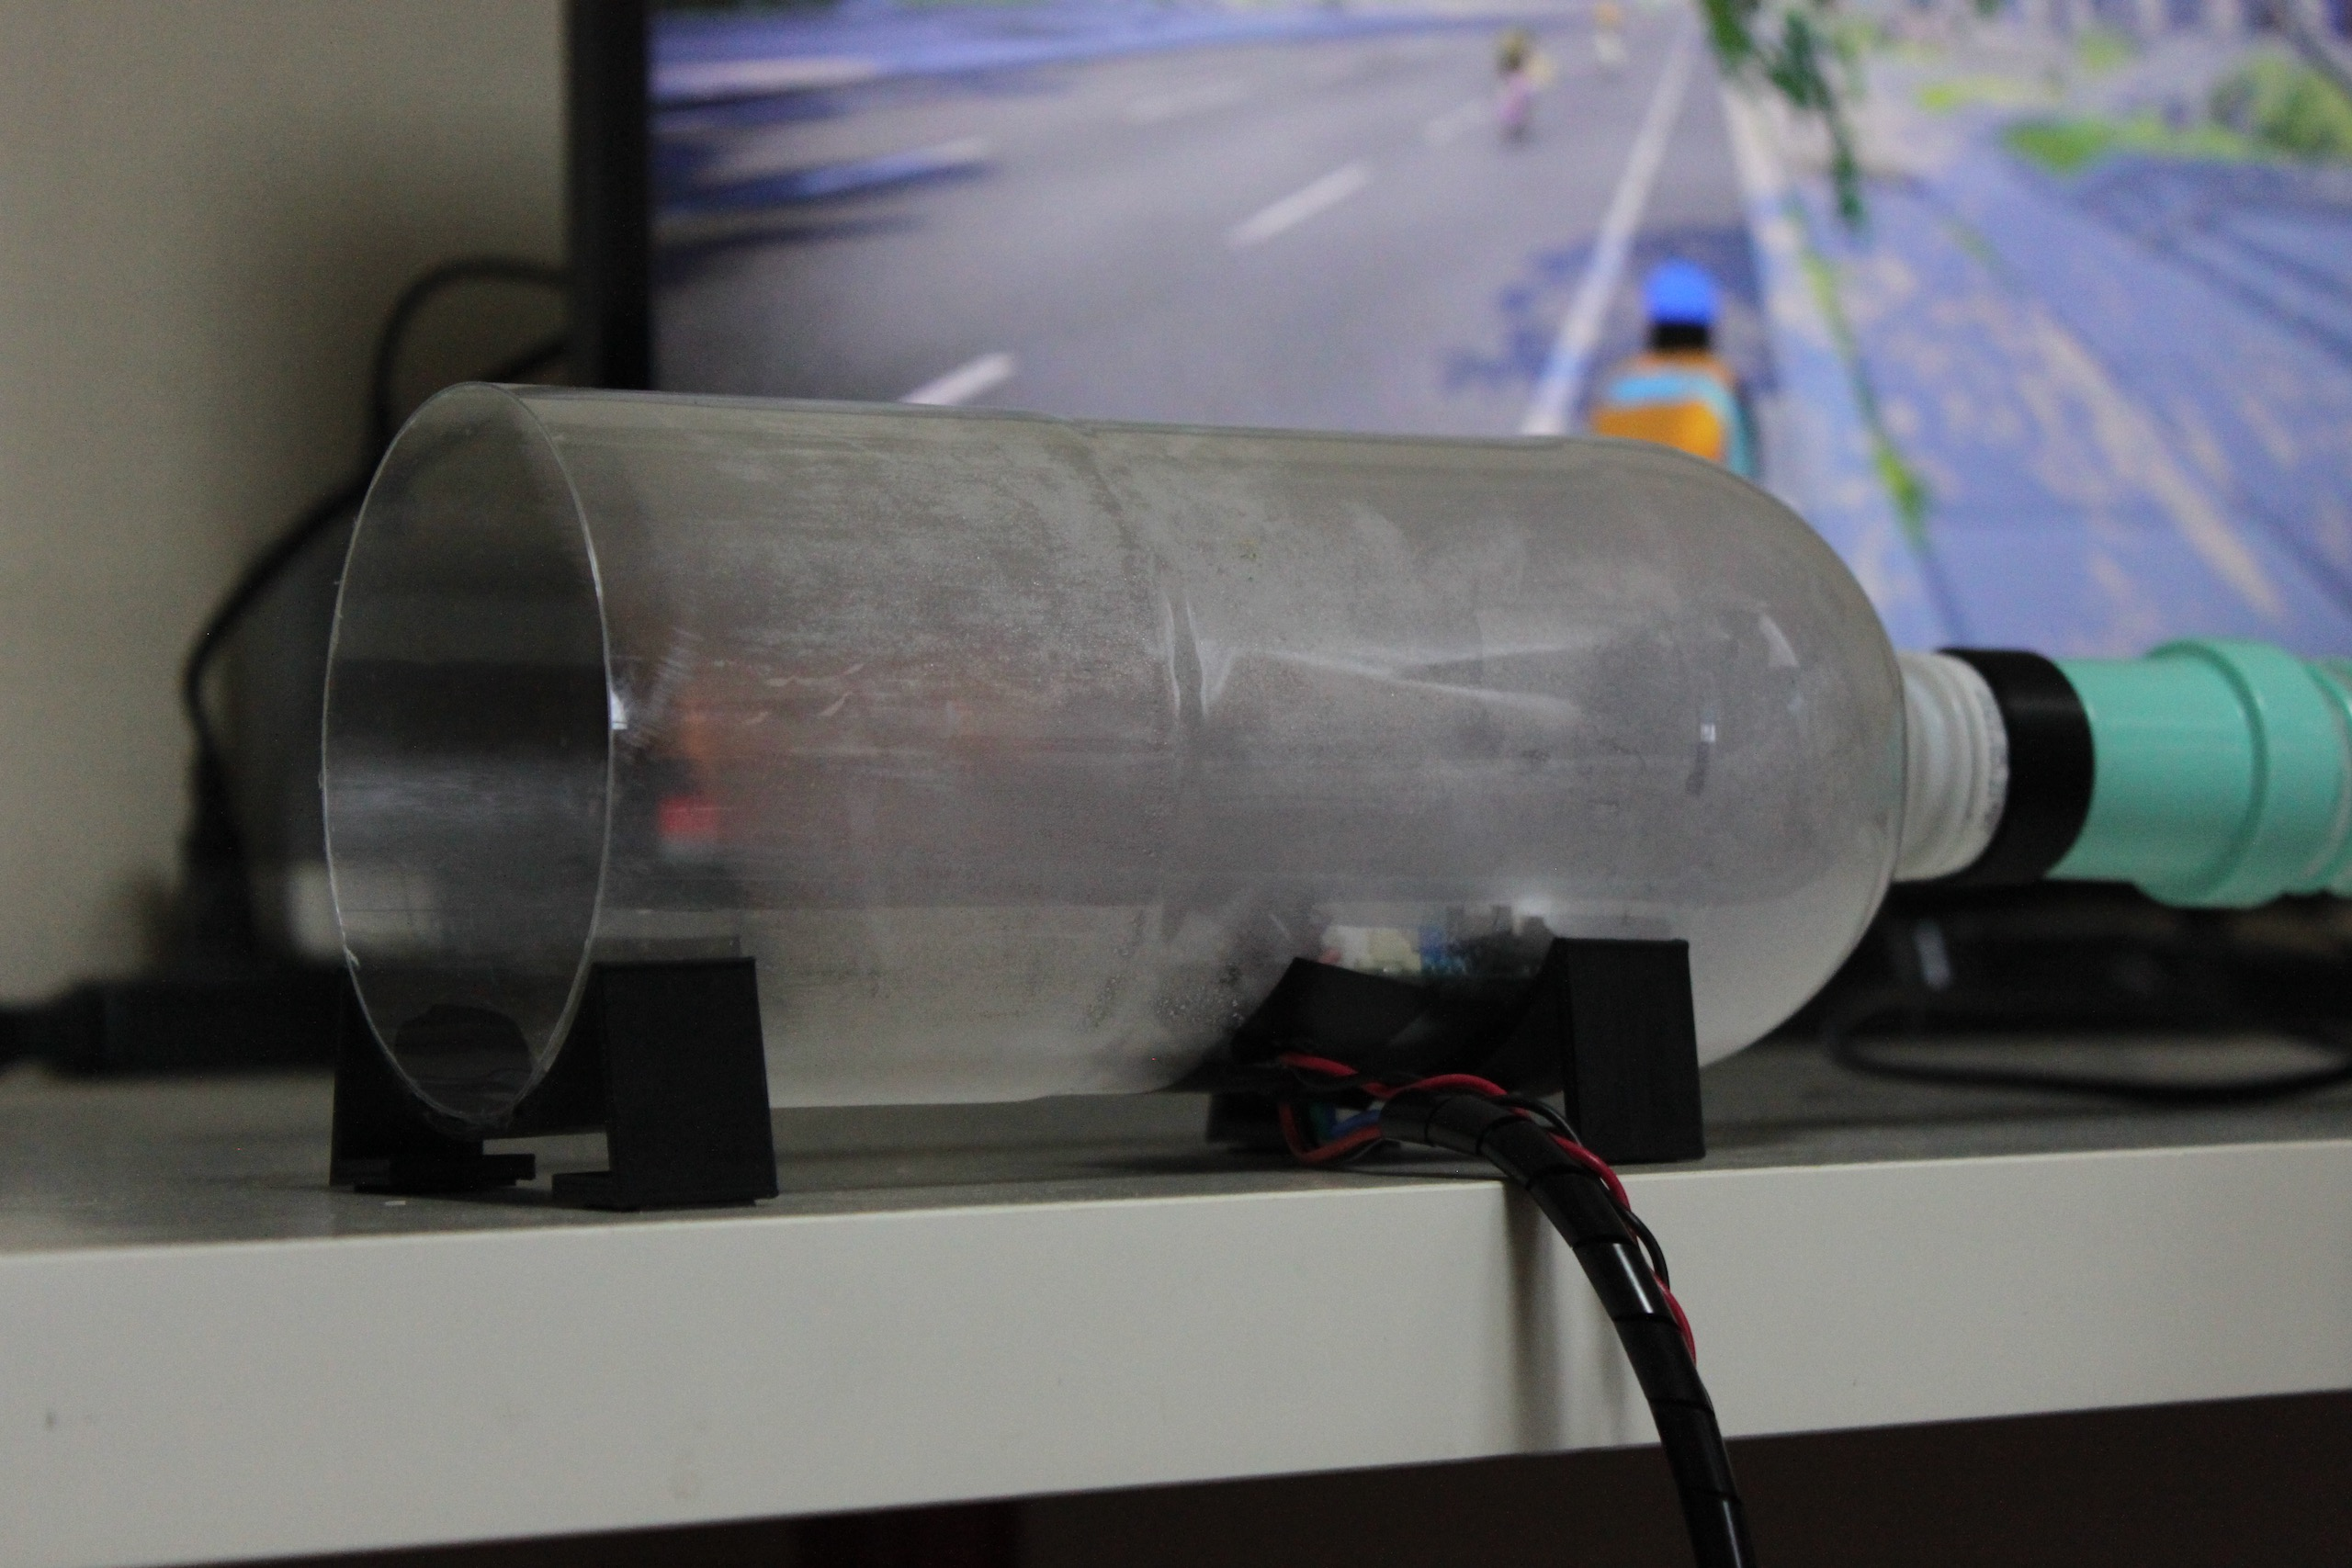
\includegraphics[width=8cm]{fig/mixing_chamber}
    \caption{製作したミキシングチャンバー}
    \label{fig:mixing_chamber}
  \end{center}
\end{figure}

図\ref{fig:mixing_chamber}は今回製作したミキシングチャンバーである.材料には入手のしやすさから1.5Lの炭酸飲料(CCレモン)のペットボトルを使用した.ミキシングチャンバーとホース(図\ref{fig:hose})を接合するためのジョイント部品はペットボトルのキャップ部のネジを使用し,ネジによる取り外し式としたものを3Dプリンターで製作した.

当初,ミキシングチャンバーは図\ref{fig:mixing_chamber_early}のように,チャンバー内のガス濃度の変化を小さくすることを意図して,ペットボトルのキャップ部同士を組み合わせて出口の流路を絞った形状としていた.しかし,実際に運動中の測定を行った場合,1分以内でチャンバー内の二酸化炭素濃度が二酸化炭素センサーの測定範囲を超えて上昇してしまうことが分かった.そこで測定中はガスの混合よりも極力外気との換気を図る必要があるということで,チャンバー内には特に障害物などを設けず,片側を解放した図\ref{fig:mixing_chamber}のような形状とした.

また,呼気ガスの成分のうち,二酸化炭素は気体標準状態において空気の2倍程度の密度があることから下方に滞留すると思われる.この際にミキシングチャンバーを置く方向が換気状況に大きく影響を与えることが予想されたので,今回はチャンバーを水平に保った状態で固定することとした.チャンバーとなるペットボトルを水平に保持できるようにするため,スタンド状の部品を3Dプリンターで製作し,センサー側の部品はネジ留めで,もう一方の部品はホットボンドで固定した.

\begin{figure}[H]
  \begin{center}
    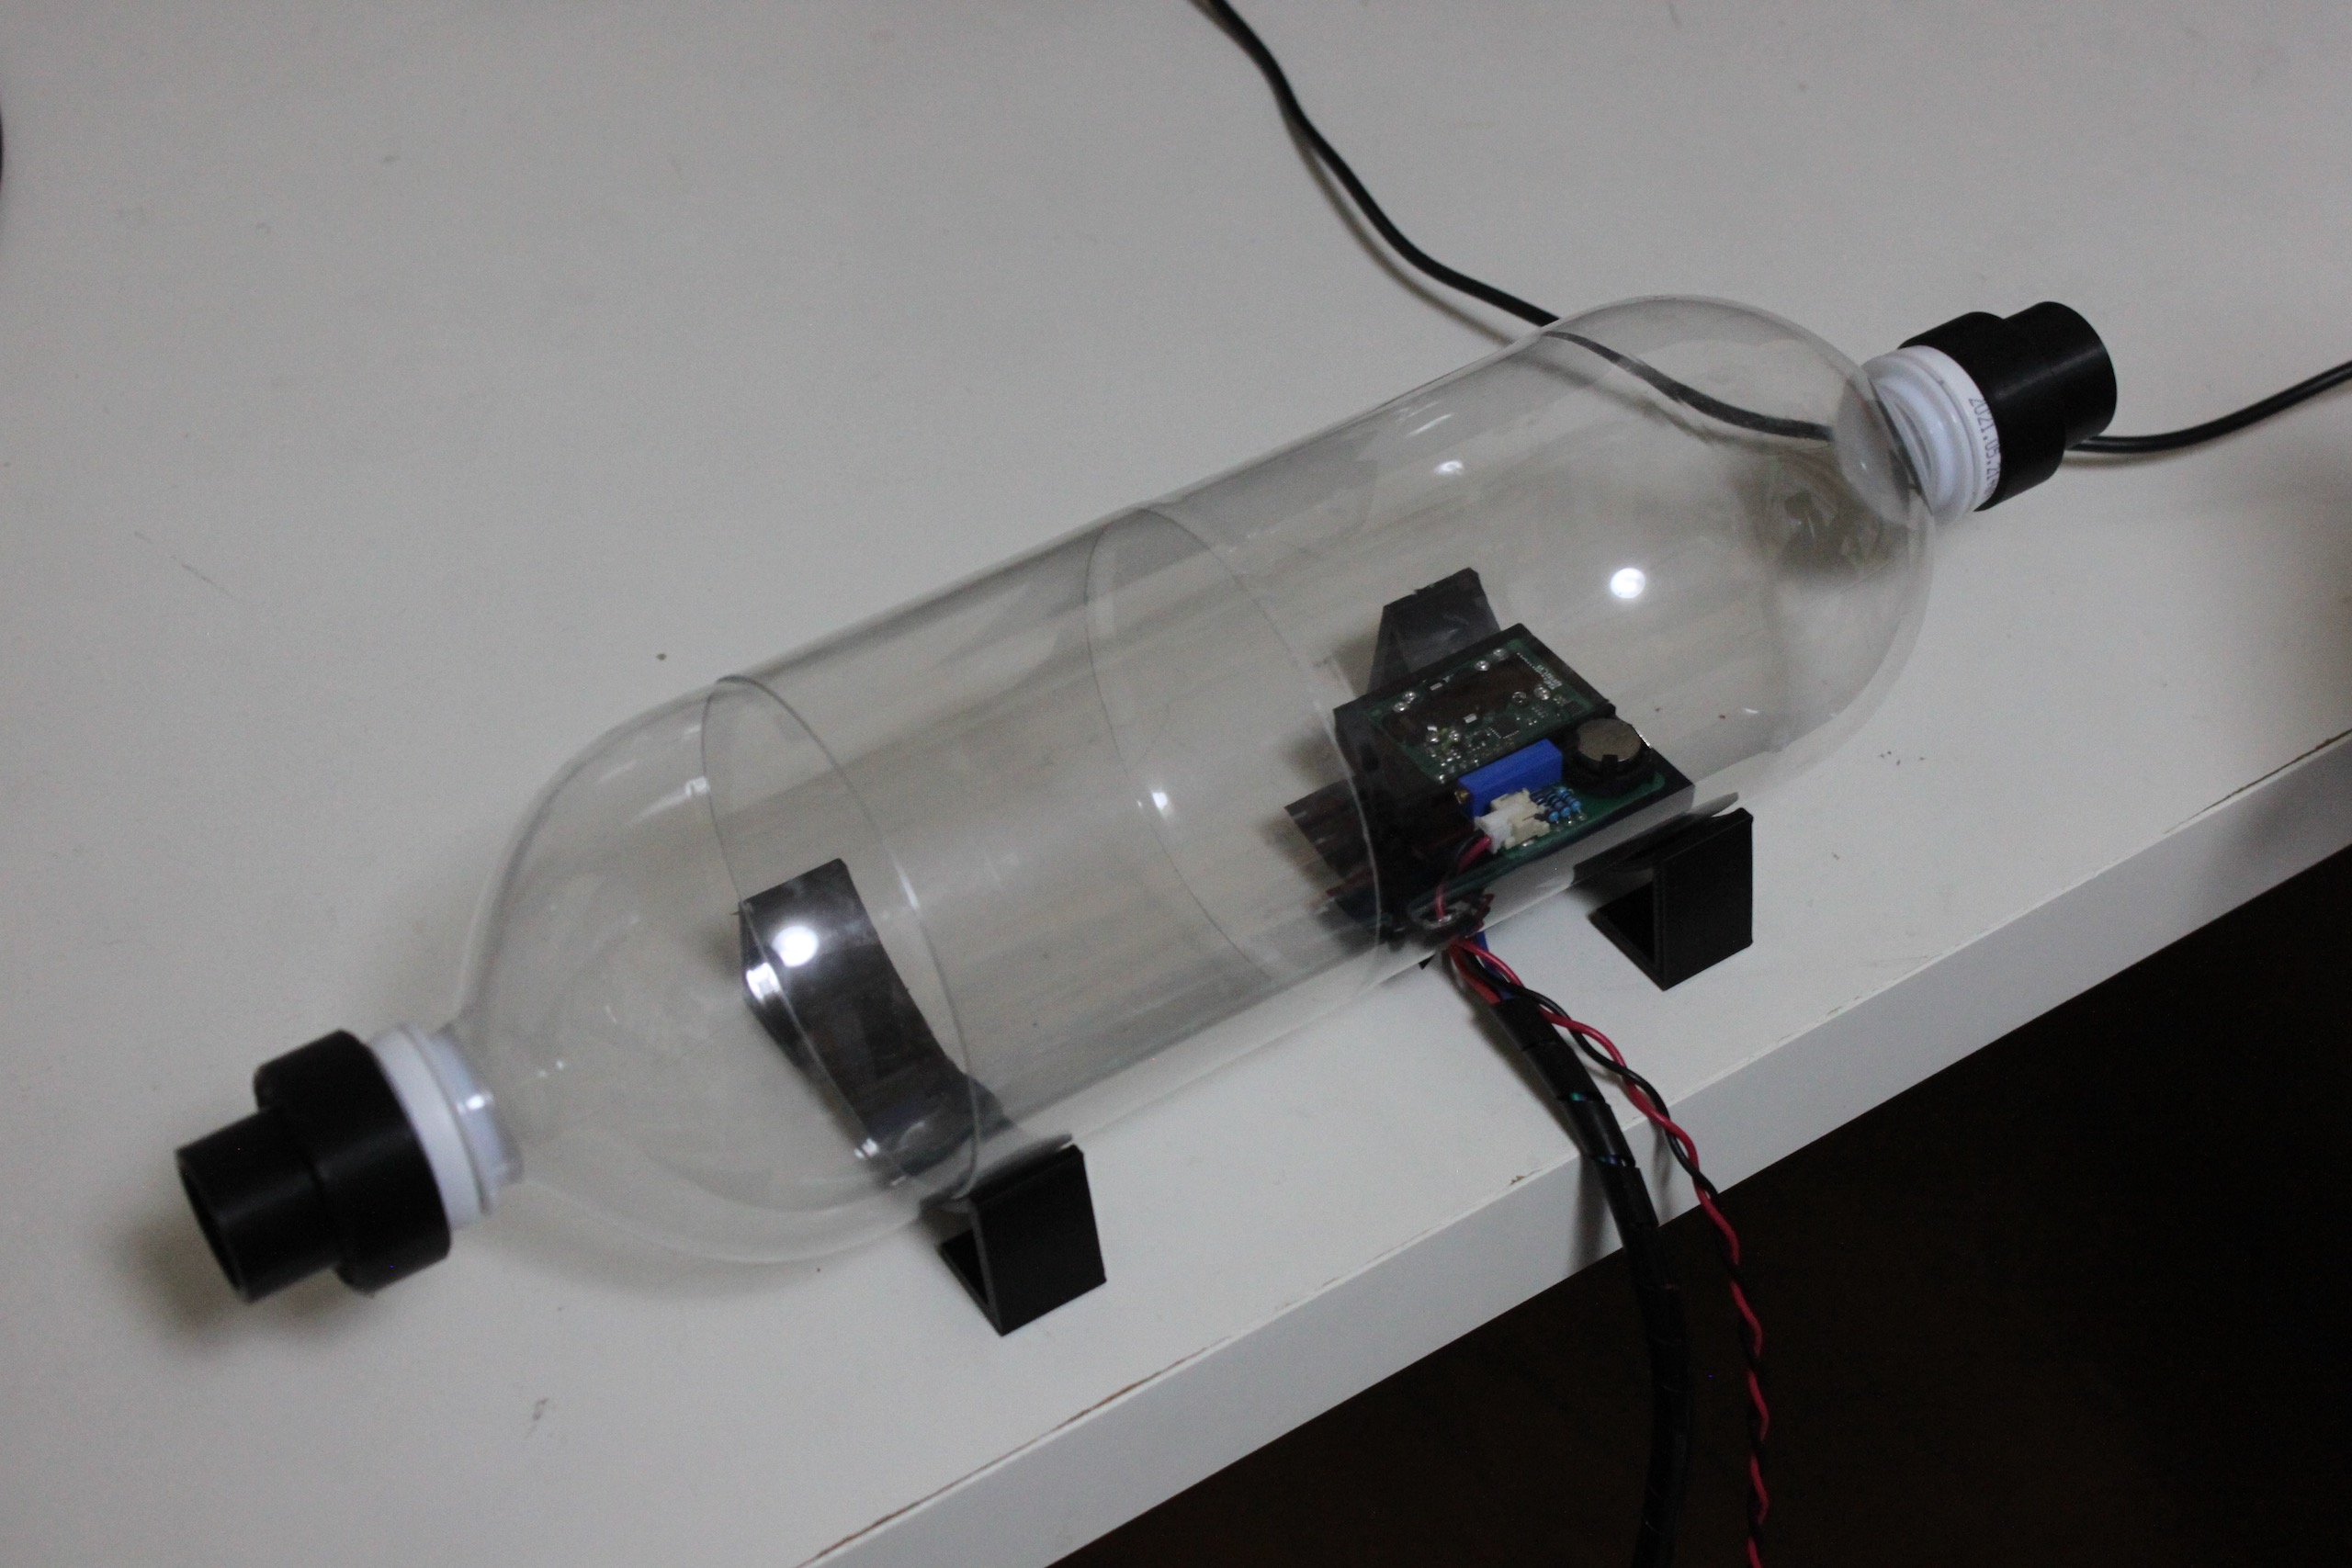
\includegraphics[width=8cm]{fig/mixing_chamber_early}
    \caption{当初のミキシングチャンバー}
    \label{fig:mixing_chamber_early}
  \end{center}
\end{figure}

\subsubsection{呼気収集マスク}

\begin{figure}[H]
  \begin{center}
    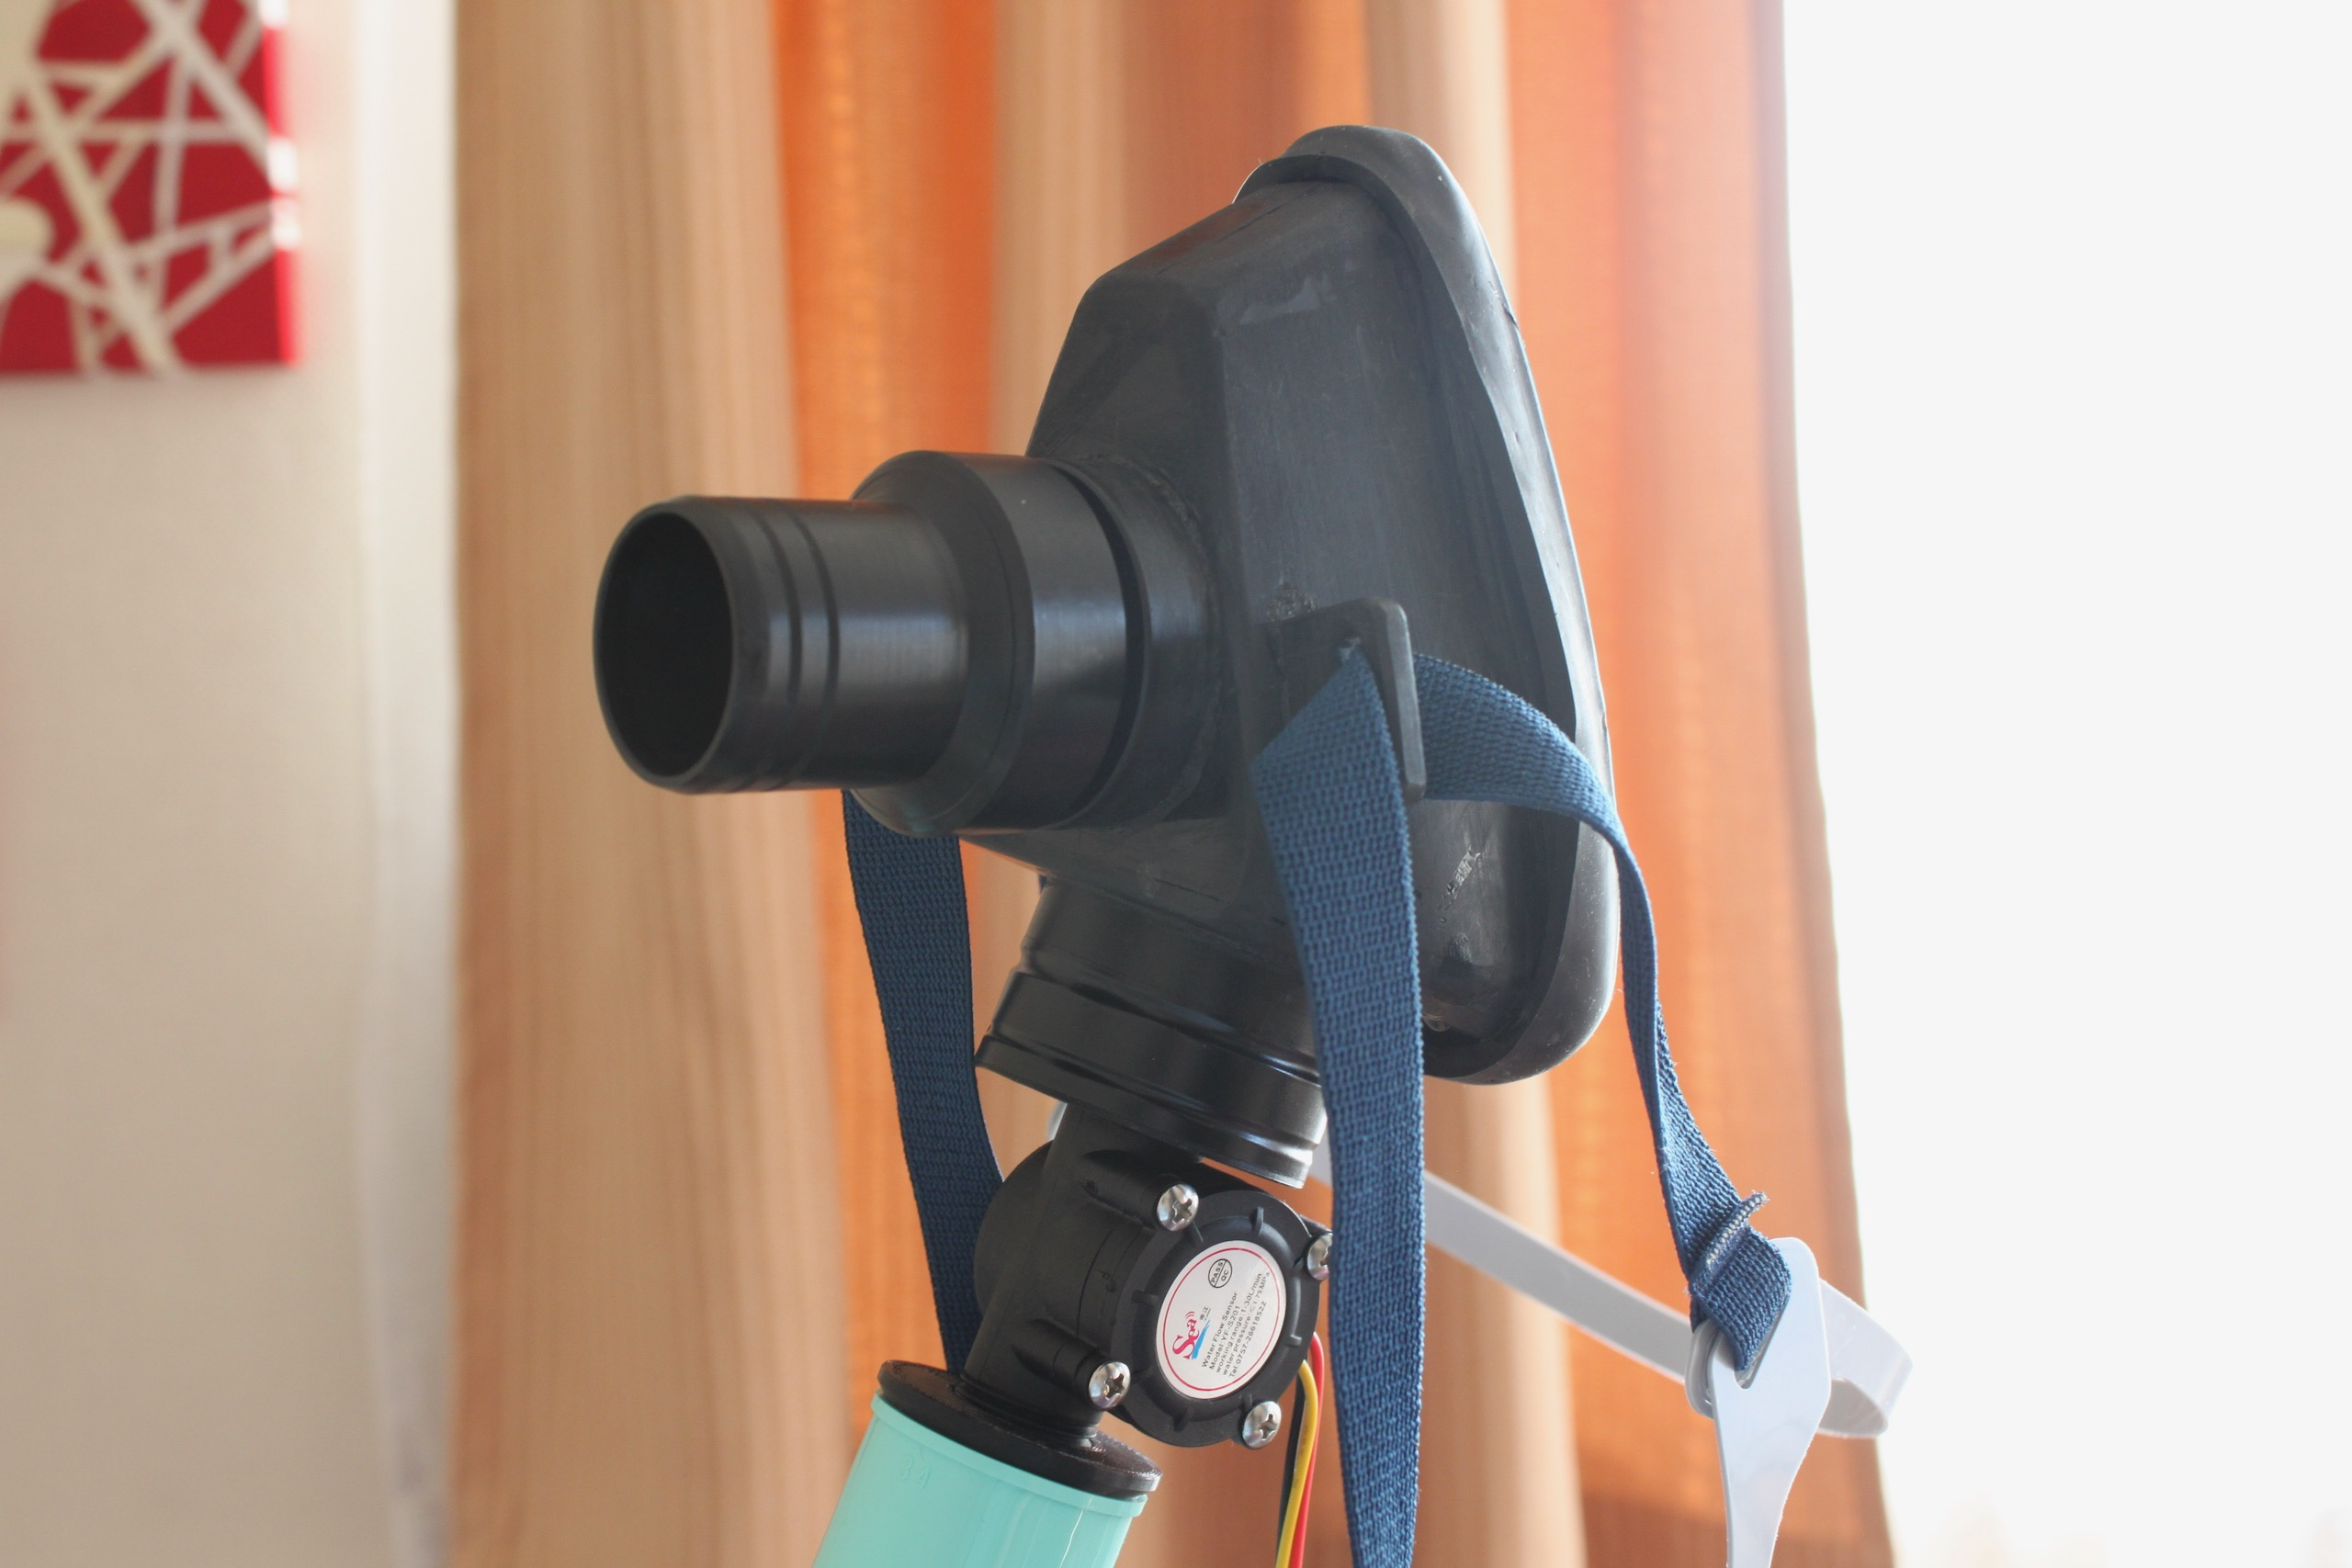
\includegraphics[width=8cm]{fig/mask_front}
    \caption{呼気収集マスク}
    \label{fig:mask_front}
  \end{center}
\end{figure}

呼気を収集するためには,呼吸の際の吸気と呼気を分離して呼気を収集するためのマスクが必要となる.これをここでは呼気収集マスクと呼ぶことにする.今回は呼気収集マスクには仰木研究室で以前に製作されたマスク(図\ref{fig:mask_front})を流用した.これは,アクリル板を組み合わせて顔に合うような形状を構成し,呼気及び吸気用の通気口を取り付けた物である.使用時に両手が使えるように,頭に固定するための市販のガスマスクから流用したバンドが取り付けられている.マスクの内側の顔に触れる部分には,顔との間にできる隙間を埋め呼気ガスが呼気の通気口以外から漏れ出すことを防ぐためのシリコーンゴム製のパッドが取り付けてある図(\ref{fig:mask_rear}).

\begin{figure}[H]
  \begin{center}
    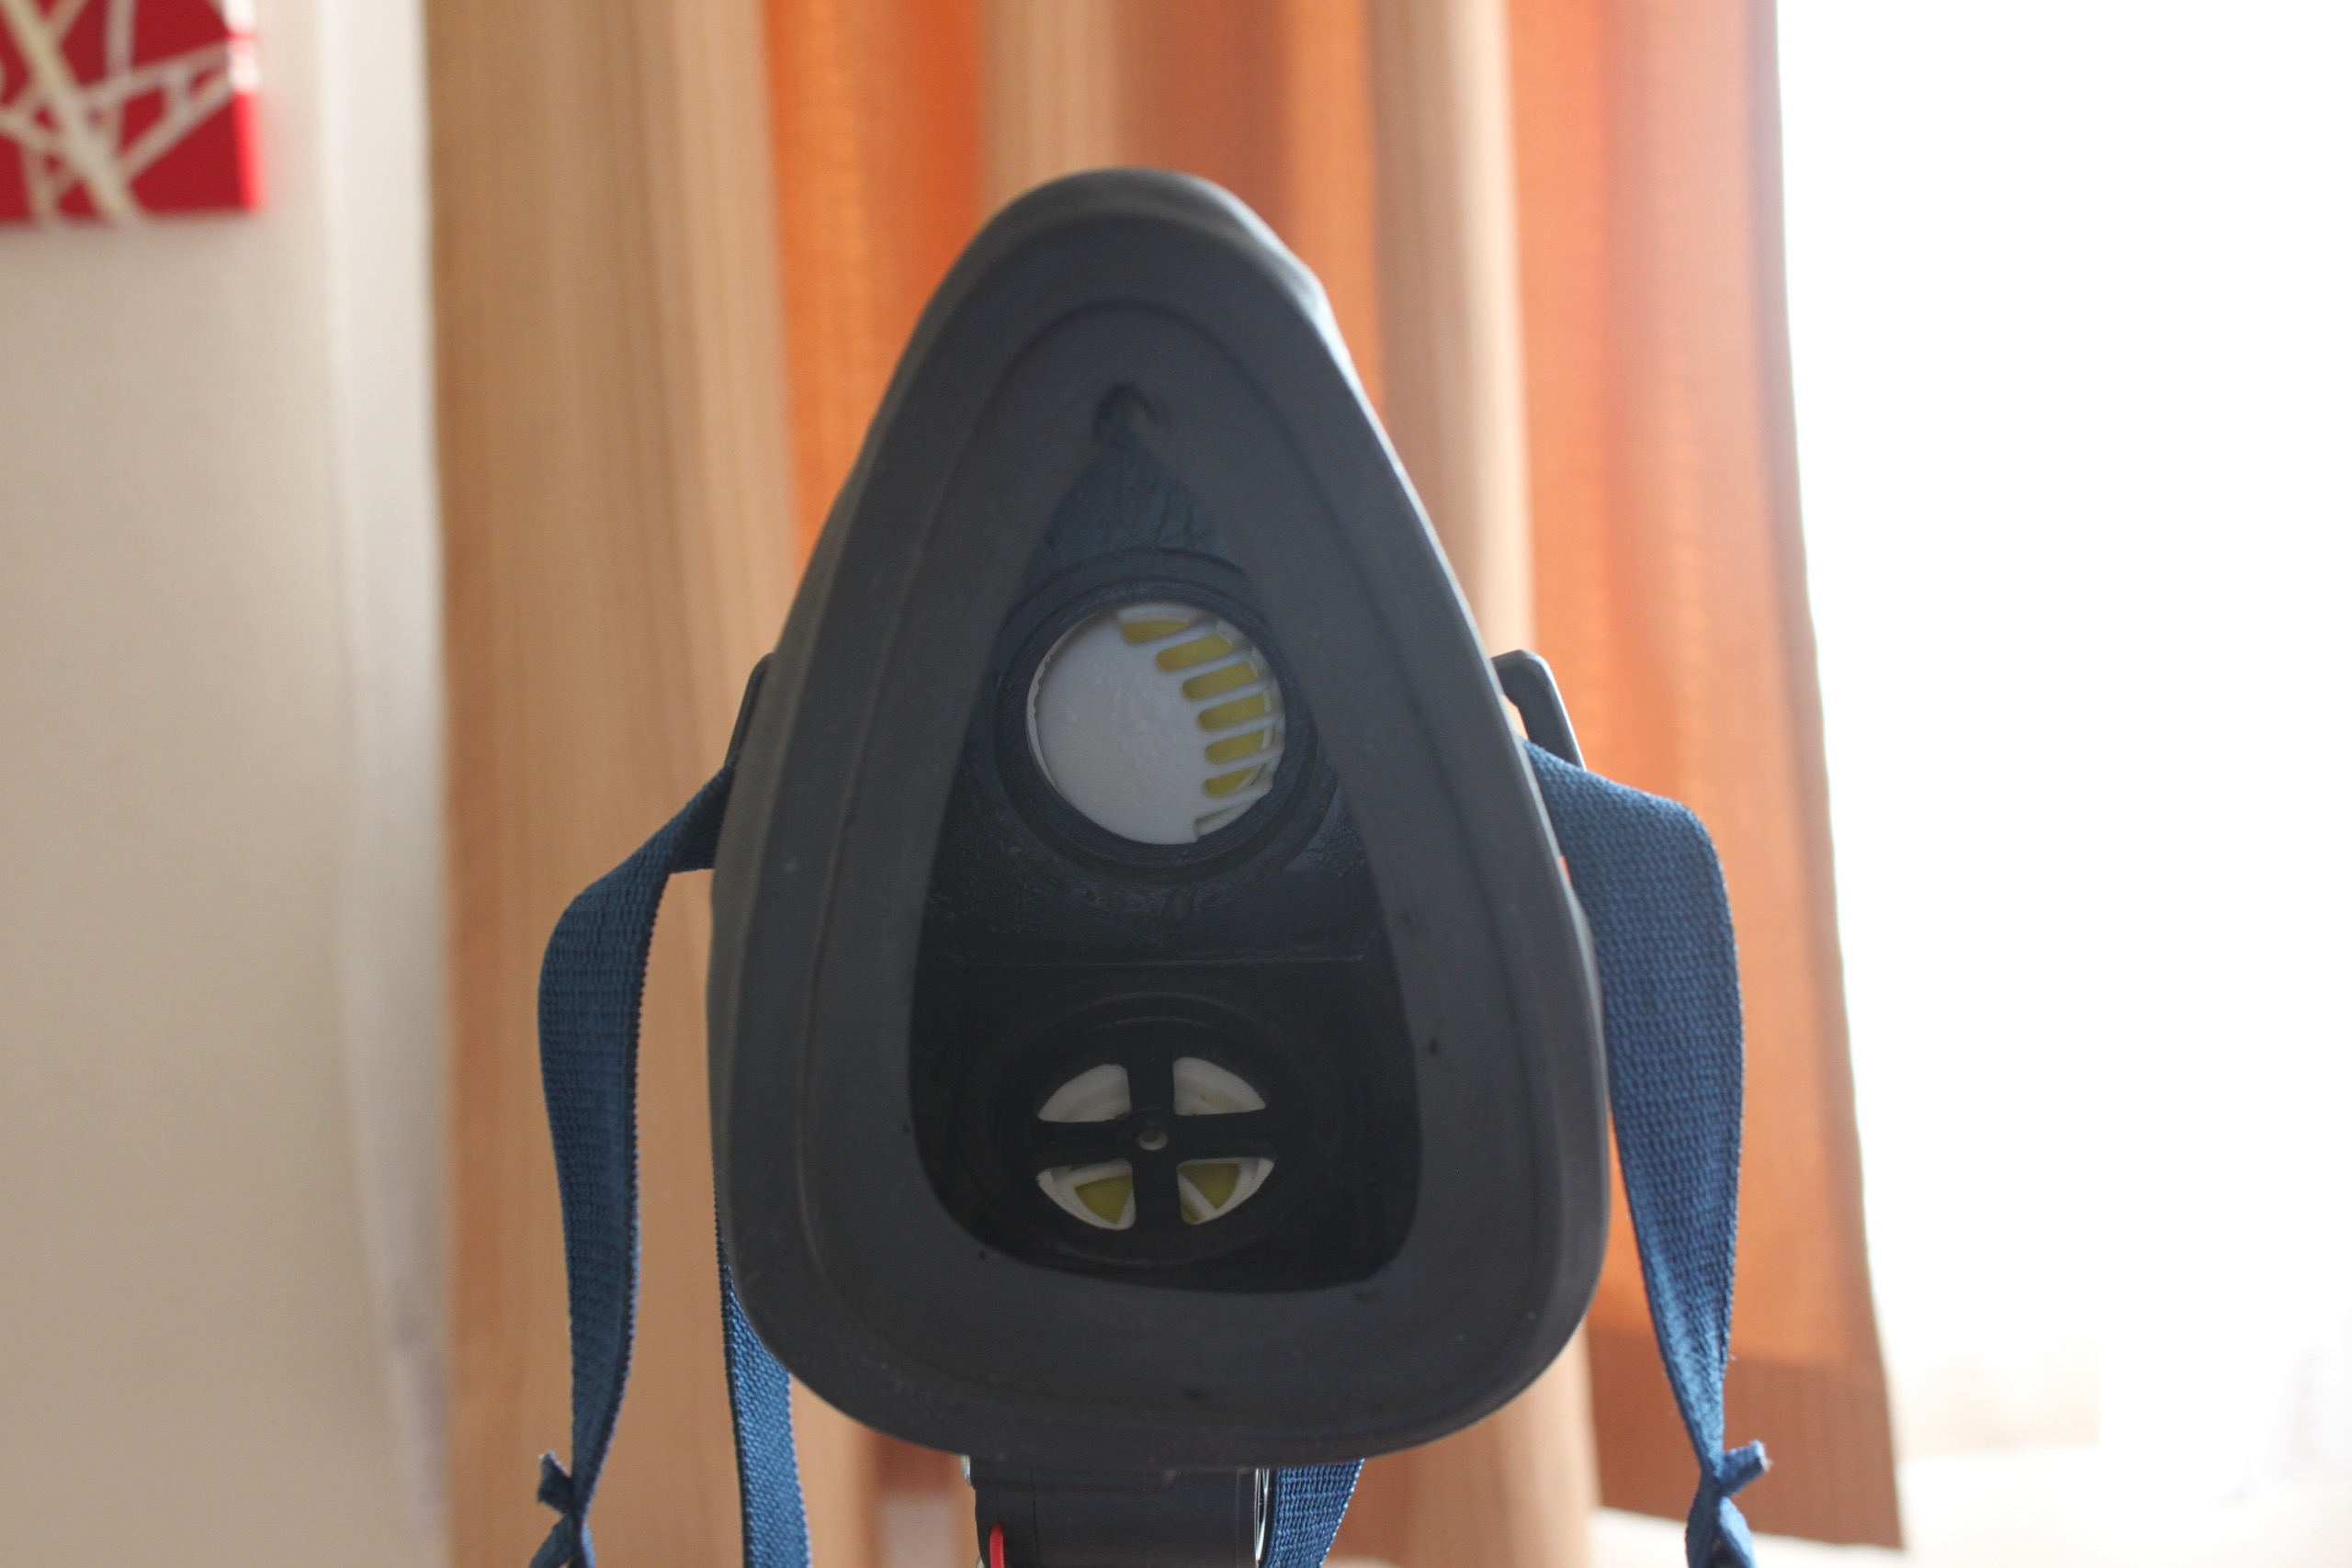
\includegraphics[width=8cm]{fig/mask_rear}
    \caption{内側から見た呼気収集マスク}
    \label{fig:mask_rear}
  \end{center}
\end{figure}

マスクの内側には,吸気と呼気を分離するために逆流防止弁を取り付けた(図\ref{fig:mask_rear}).なお,一般的なガスマスクに倣い,今回は鼻の前あたりに位置する前方向の通気口を吸気,口の前下あたりに位置する下方向の通気口を呼気とした.今回使用した逆流防止弁は,運動時に使用するマスクに取り付けるために安価に市販されている物である.逆流防止弁の構造は図\ref{fig:bulb}のようになっている.ごく薄いシリコーンゴム製の膜は,一方向のみに捲れることができるようにプラスチック製の2つのパーツに挟まれて取り付けられている.これによって,弁を流れる気体の流れる方向を一方向に制限することができる.この弁を3Dプリンターで製作したスペーサーでマスク本体の径に合わせた上でネジで固定している.

\begin{figure}[H]
  \begin{center}
    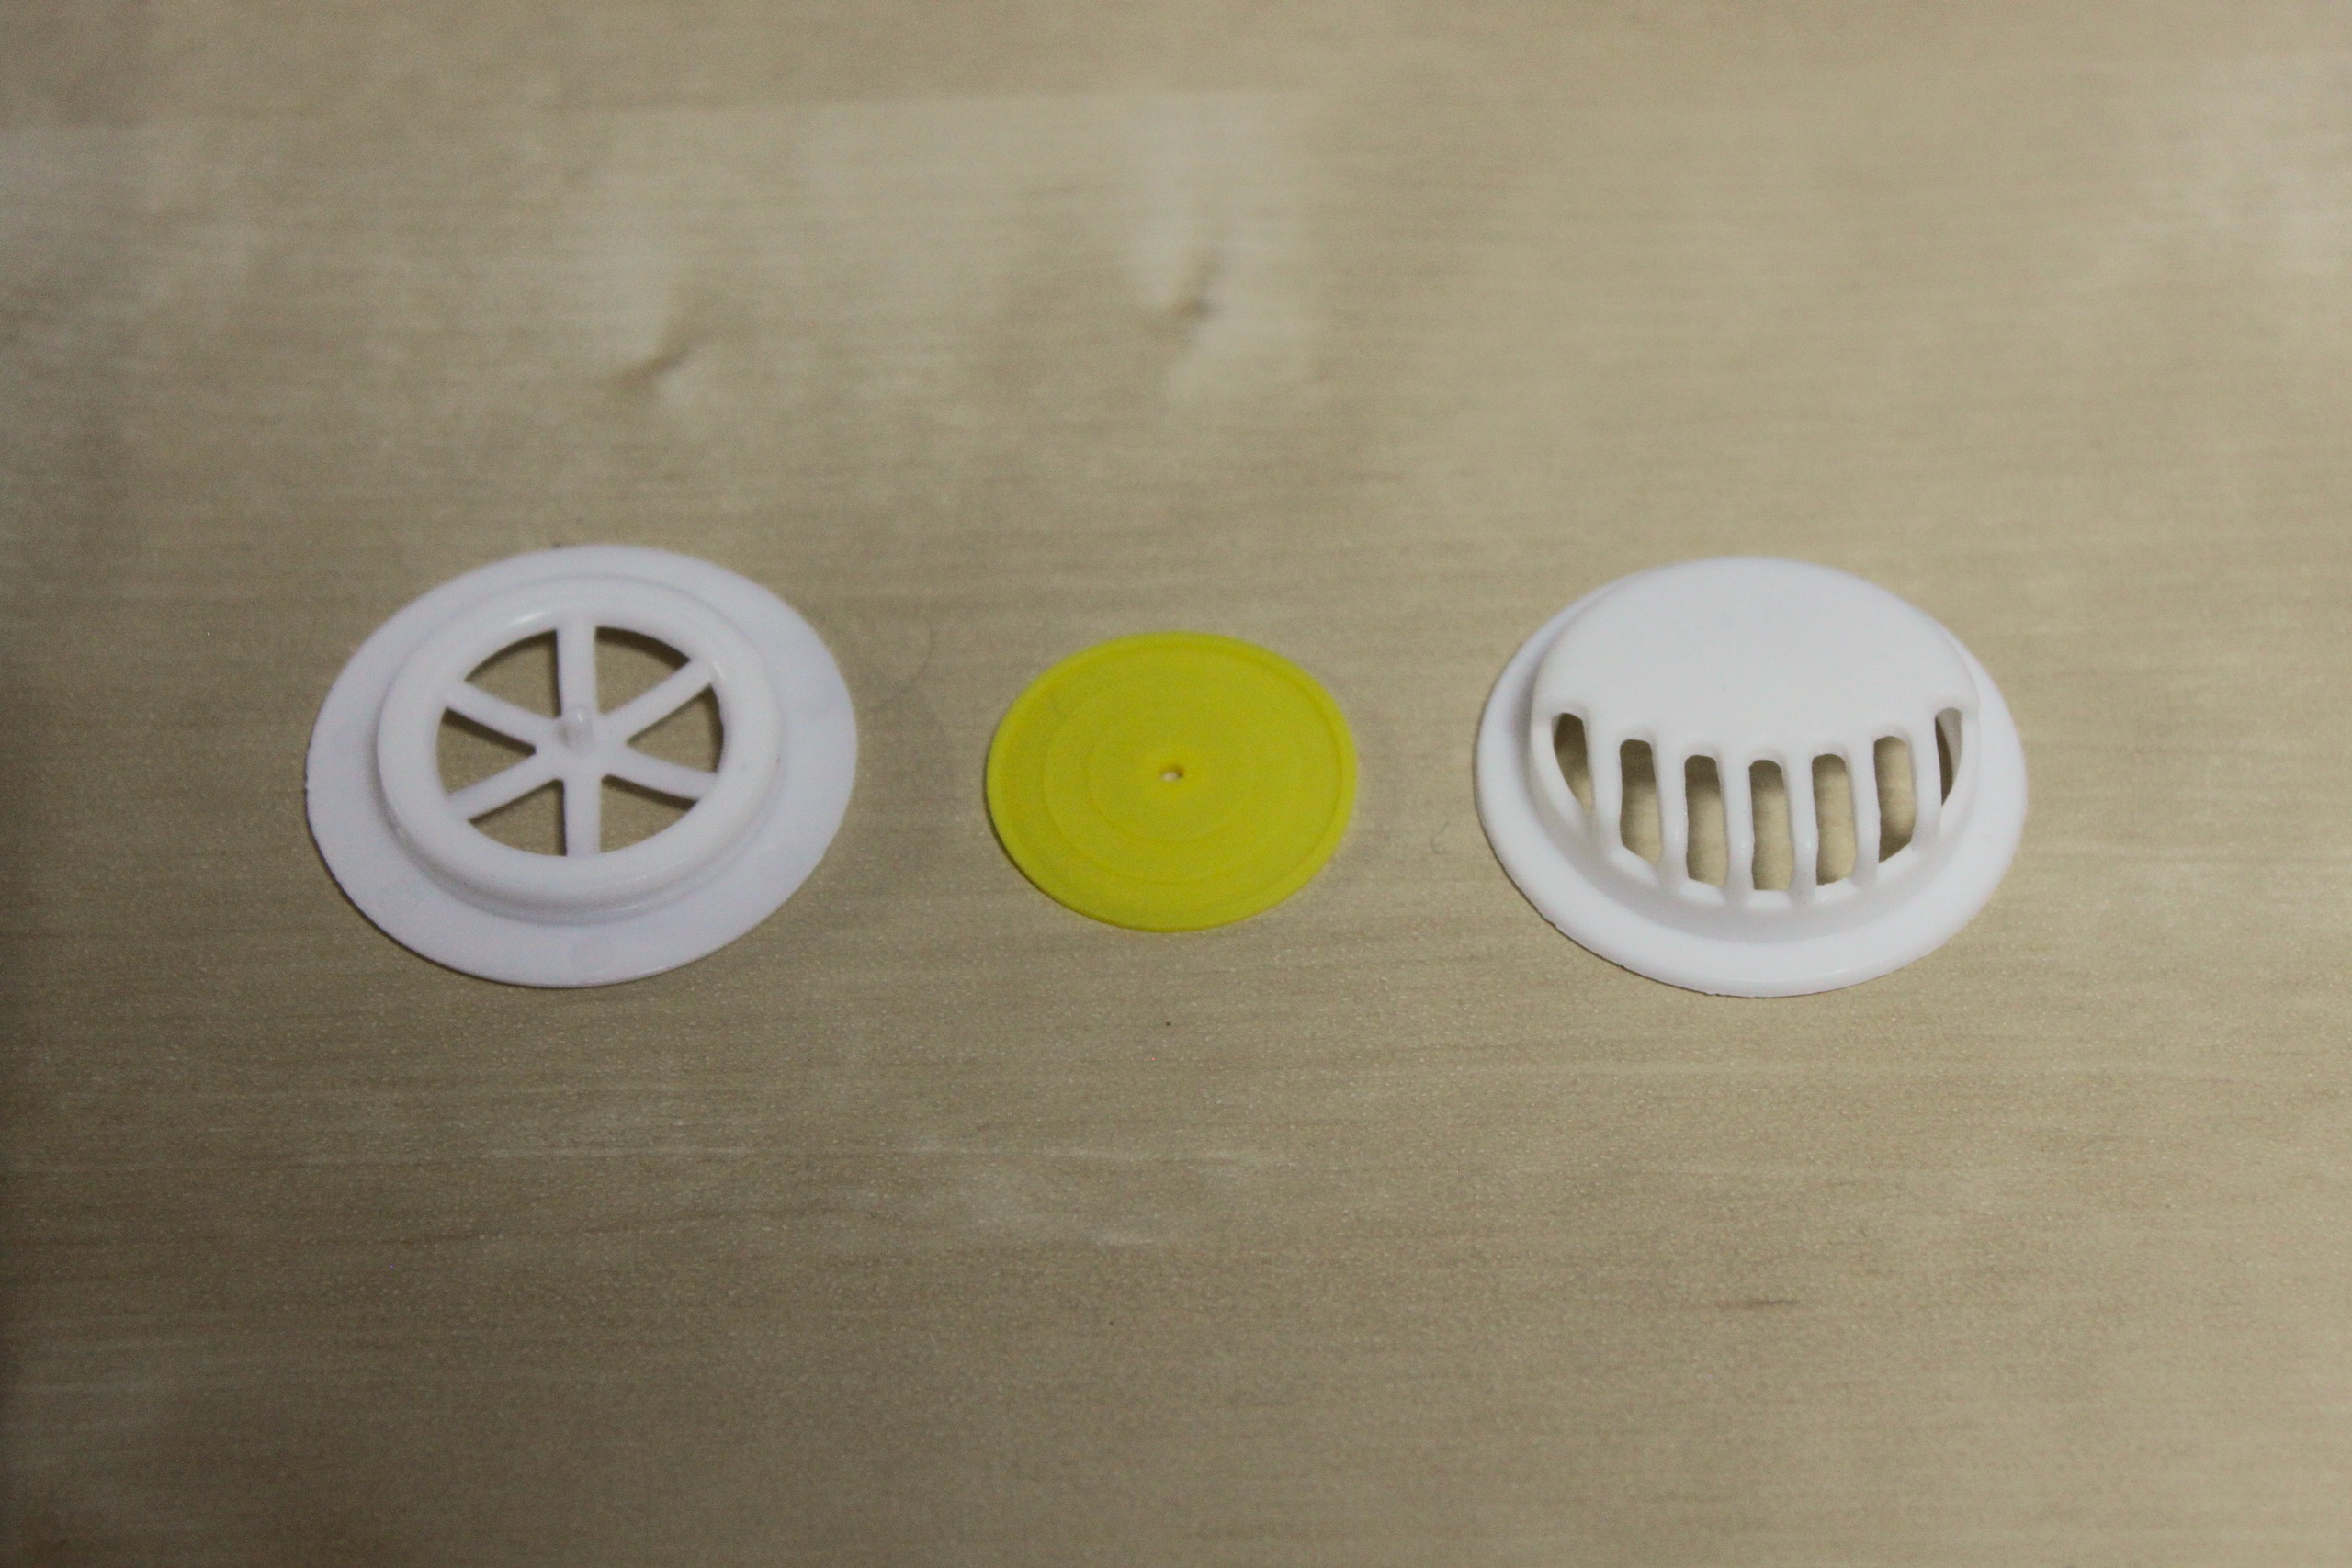
\includegraphics[width=8cm]{fig/bulb}
    \caption{逆流防止弁の構造}
    \label{fig:bulb}
  \end{center}
\end{figure}

ミキシングチャンバーと呼気収集マスクを接続するためのホースには,洗濯機の排水用ホースの延長ホースとして市販されている物(図\ref{fig:hose})を使用した.このホースは内径30mmの塩化ビニル製で,片側がゴム製,もう片側が硬質プラスチック製の継手となっている.今回はチャンバー側にプラスチック製,マスク側にゴム製の継手を接続することにし,ジョイント部品を3Dプリンターで製作した.

\begin{figure}[H]
  \begin{center}
    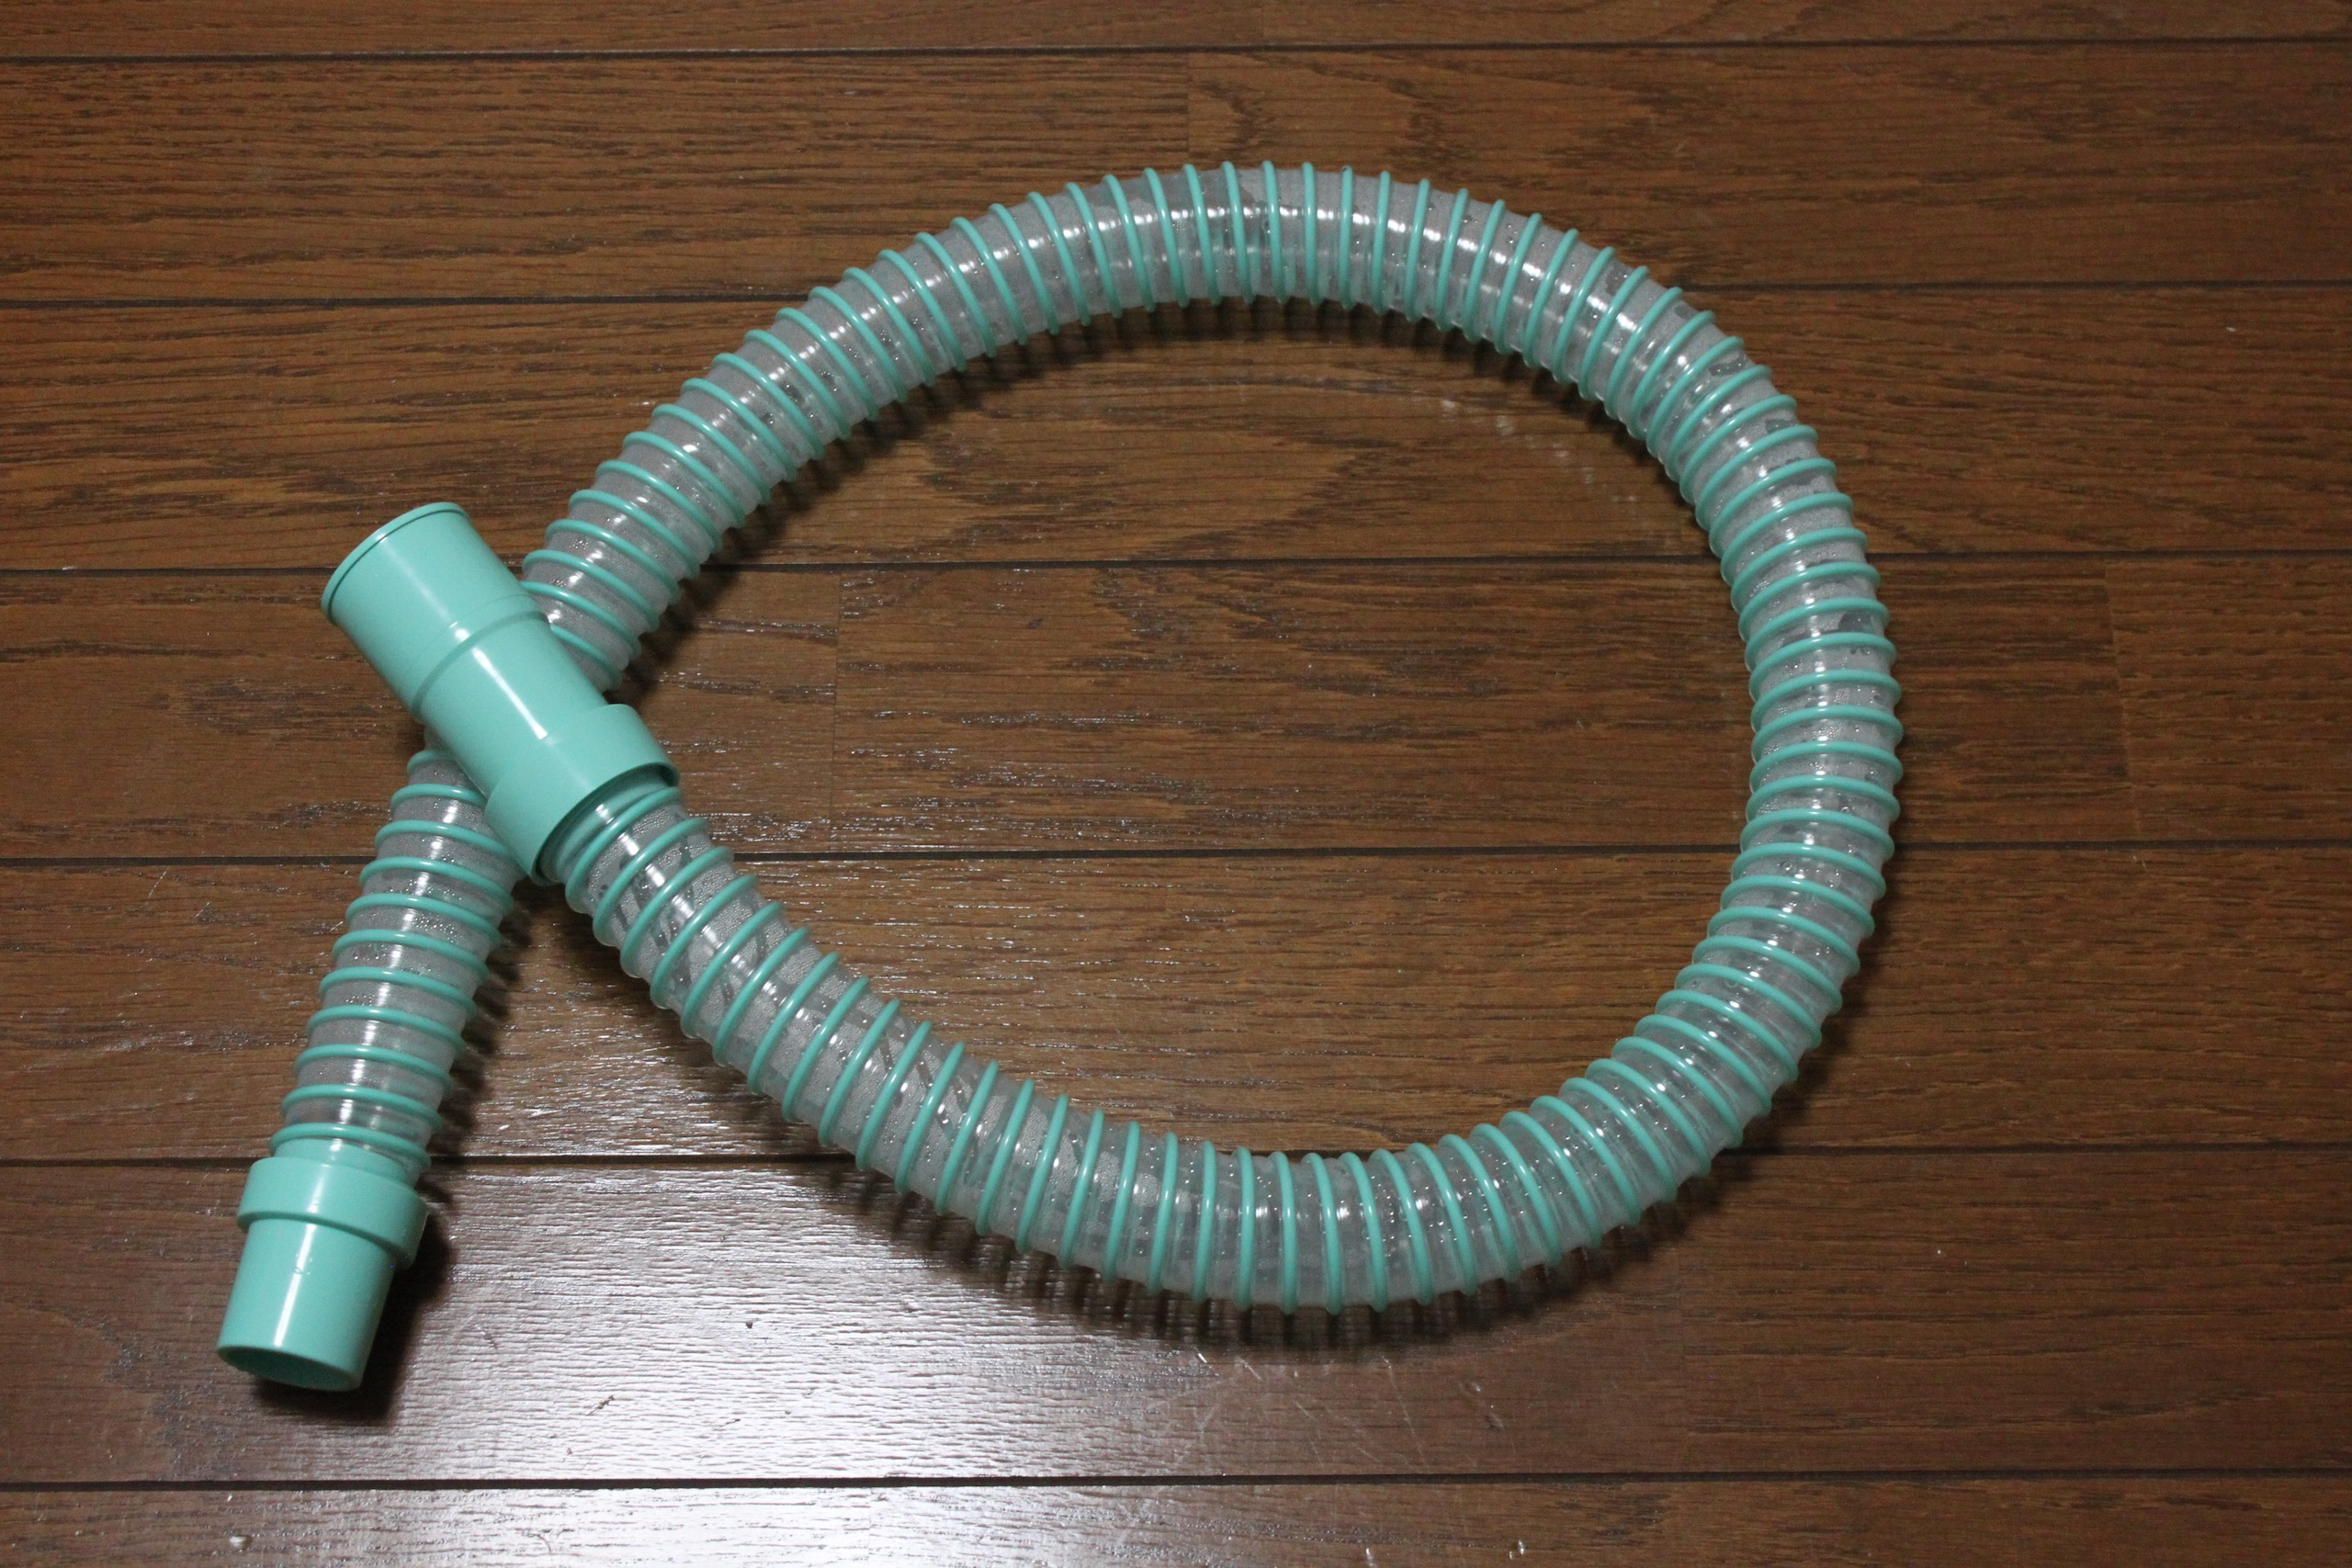
\includegraphics[width=8cm]{fig/hose}
    \caption{洗濯ホース}
    \label{fig:hose}
  \end{center}
\end{figure}

\subsection{換気量の測定}

\subsubsection{計測方式}

\ref{sec:correct}に述べたように,今回はミキシングチャンバー方式で呼気を収集する.ミキシングチャンバー法では,換気量の測定を呼気の流路に流量計を設置することで収集中に行う必要がある.

気体の流量を測定するための流量計の原理としては,差圧流量計と超音波流量計,タービン流量計などがある.各方式の特徴を表\ref{tb:flowsensor_method}にまとめた.

\begin{table}[H]
\begin{center}
\caption{主な気体流量計の測定方式}
\label{tb:flowsensor_method}
\begin{tabular}{|l|l|l|}
\hline
 & 原理 & 構造 \\ \hline
差圧流量計   & \begin{tabular}[c]{@{}l@{}}流路内に流路を絞った機構を設ける.\\ その前後に発生する圧力差を測定する.\end{tabular}    & 微細     \\ \hline
超音波流量計  & \begin{tabular}[c]{@{}l@{}}流路内の液体に超音波を照射する.\\ 照射した超音波の反射によって流量を測定する.\end{tabular} & 微細     \\ \hline
タービン流量計 & \begin{tabular}[c]{@{}l@{}}流路内にタービンを設置する.\\ タービンの回転数によって流量を測定する.\end{tabular}     & 微細ではない \\ \hline
\end{tabular}
\end{center}
\end{table}

差圧流量計は流路内に絞り機構を設け,その前後に発生する圧力差を測ることで流量を計測する方式である.超音波流量計は,流路内を流れる流体に超音波を照射することで流量を計測する方式である.タービン流量計は,流路にタービンを設置し,流体によって回転するタービンの回転数によって流量を計測する方式である.

気体流量計はいずれの方式も高価な部品である.呼吸代謝測定装置の製作において,流量計のコストを抑えることは大きな課題であると言える.タービン流量計は単純な構造であり,他の方式に比べて微細ではない構造なので,水流計として安価に市販されている.今回は研究の趣旨として,呼吸代謝測定装置としての最高性能を多少損なったとしても,装置全体の全体の価格を抑えることの優先順位が高いと考えたためにタービン流量計を使用した.

今回使用した水流計はYF-S201という名称で市販されているもので,流路に対してタービンの軸が垂直に取り付けられている接線流羽根車式のタービン流量計である.タービンの回転数に応じてホール素子が矩形波の信号を出力する.YF-S201と主な仕様を図\ref{fig:yf-s201}と表\ref{tb:YFS201_specsheet}に示す.

\begin{figure}[H]
  \begin{center}
    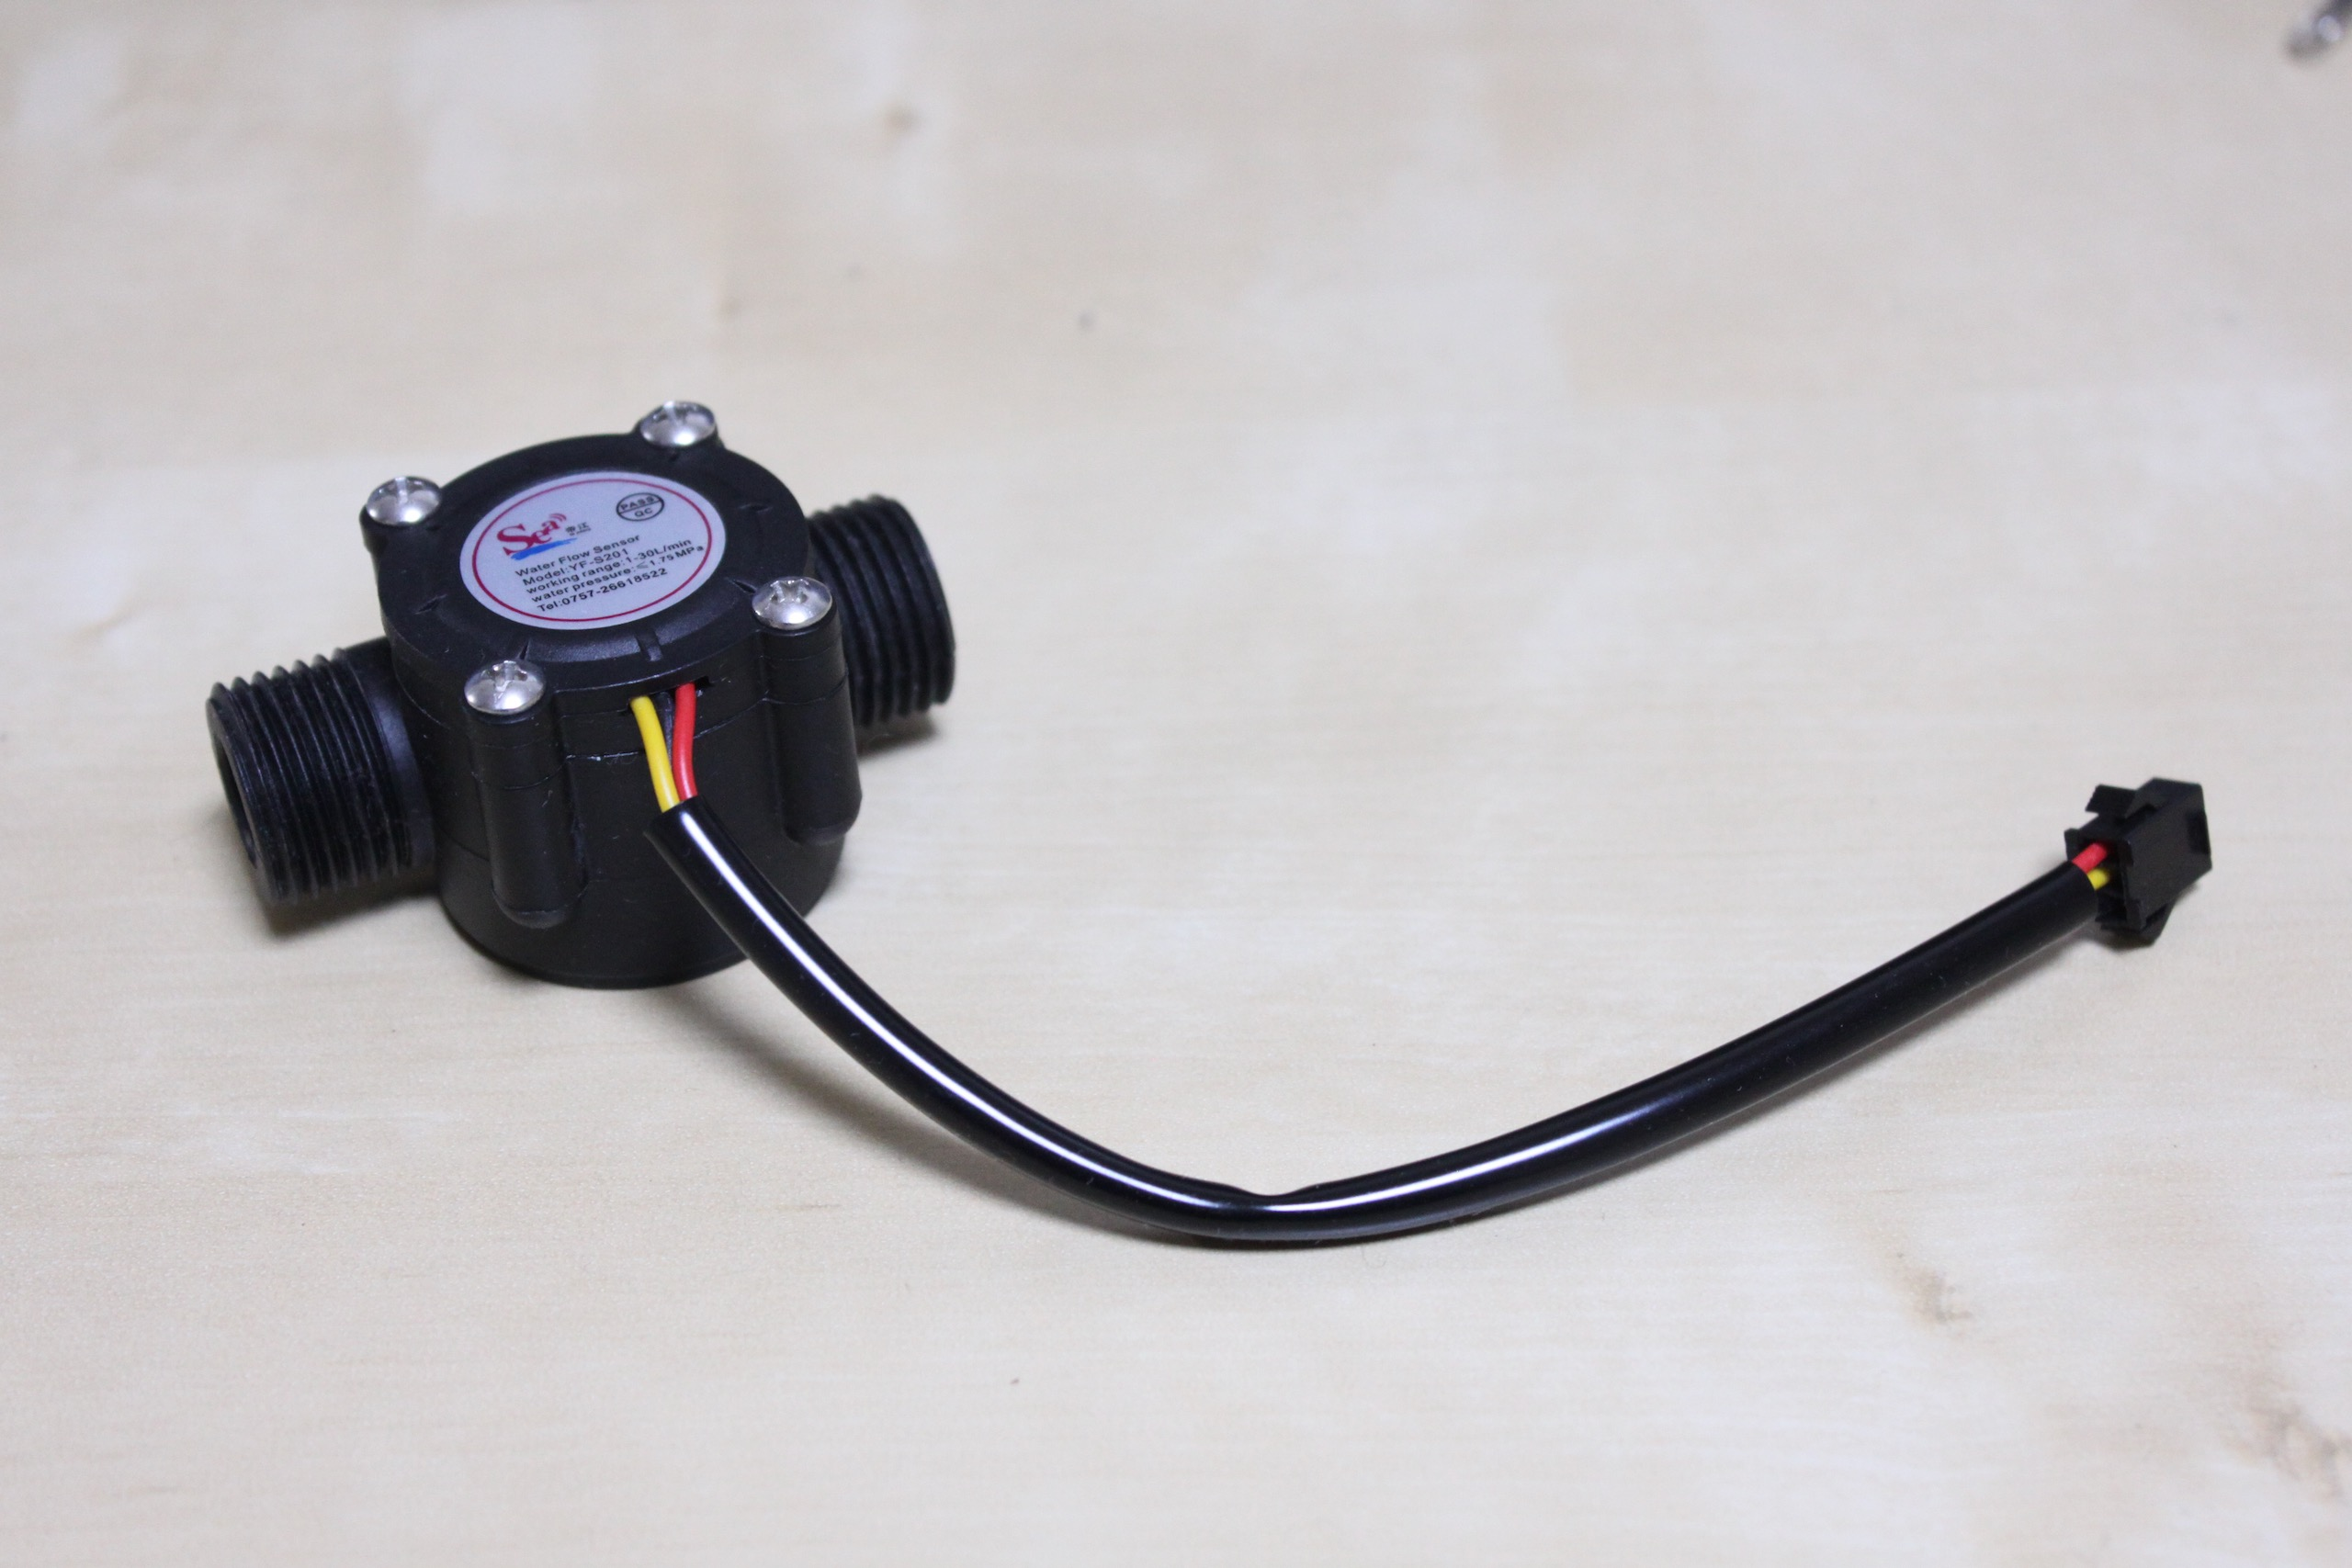
\includegraphics[width=8cm]{fig/yf-s201}
    \caption{水流計 YF-S201}
    \label{fig:yf-s201}
  \end{center}
\end{figure}

\begin{table}[H]
\begin{center}
\caption{YF-S201 主な仕様}
\label{tb:YFS201_specsheet}
\begin{tabular}{|l|l|}
\hline
回転数測定方式 & ホール素子                    \\ \hline
本体素材    & PVC                      \\ \hline
インペラ素材  & POM                      \\ \hline
重量      & 49.5g(実測値)               \\ \hline
流路外径    & 20mm                     \\ \hline
流路入口内径  & 9mm                      \\ \hline
流路出口内径  & 12mm                     \\ \hline
動作流量    & 1-30L/min                \\ \hline
取付角度    & 90度\pm5度                 \\ \hline
流量-パルス  & 1L_{水}/min = 450_{pulse} \\ \hline
\end{tabular}
\end{center}
\end{table}

\ref{sec:correct_method}で述べたように,最大作業の測定を行う場合には呼気が流れる流路の内径は35mm以上必要であるという.今回使用したYF-S201は最小径が9mmとなっているため,必要とされる35mmの場合に比べて断面積比で7\%程度の流路断面積となっていることになる.このことから,今回製作した装置は最大作業の測定には使用できないことが分かる.今回は{\bf 最大作業の測定を考慮しない代わりに呼吸代謝測定装置を安価に製作することが目的}である.また,実際に流路径が足りない装置で実際に運動中の呼吸代謝測定装置を行った場合の使用感の検証も行うことも目的とする.

\subsubsection{タービン式流量計の空気流量係数の測定}

表\ref{tb:YFS201_specsheet}の仕様によれば,YF-S201は1分あたり水流1Lが流路を流れる時に1分あたり450個の矩形波を出力する.ただし,これは水流が流れる時の値なので,空気の流量計として使用するためには空気が流れる際の関係式を求める必要がある.また,使用する呼気収集マスク\ref{fig:mask_front}に水流計を取り付けた際に,取付角度は仕様の90度\pm5度を逸脱し,顔が正面を向いた状態で60度程度となる.そこで,今回は取付角度が60度の場合に流体として空気が流れる場合の流量-パルス値を実験で求めた.

今回は流量計を図\ref{fig:mask_front}のように逆流防止弁の先に取り付ける.また,呼気の流量は一呼吸の内,吸気が終了した時点の0から最も強く息を吐き出す最大の範囲で常に変動する.これにより,呼気の流量は,吸気中は逆流防止弁が閉じているため0になり,呼気開始とともに逆流防止弁が開き次第に大きくなり,呼気終了時点で瞬時に0になる.そこで,一定流量の空気を流し続けた際の値を求めるのではなく,YF-S201が{\bf 一定量の空気が流れた際のパルス数が毎回等しくなるということを仮定}し,流量ではなく,パルス数あたりの流れた空気の容量を求めるための係数を算出している.この係数から流量を求めるためには,係数から求められた流れた空気の容量を時間で割ればよい.

\begin{figure}[H]
  \begin{center}
    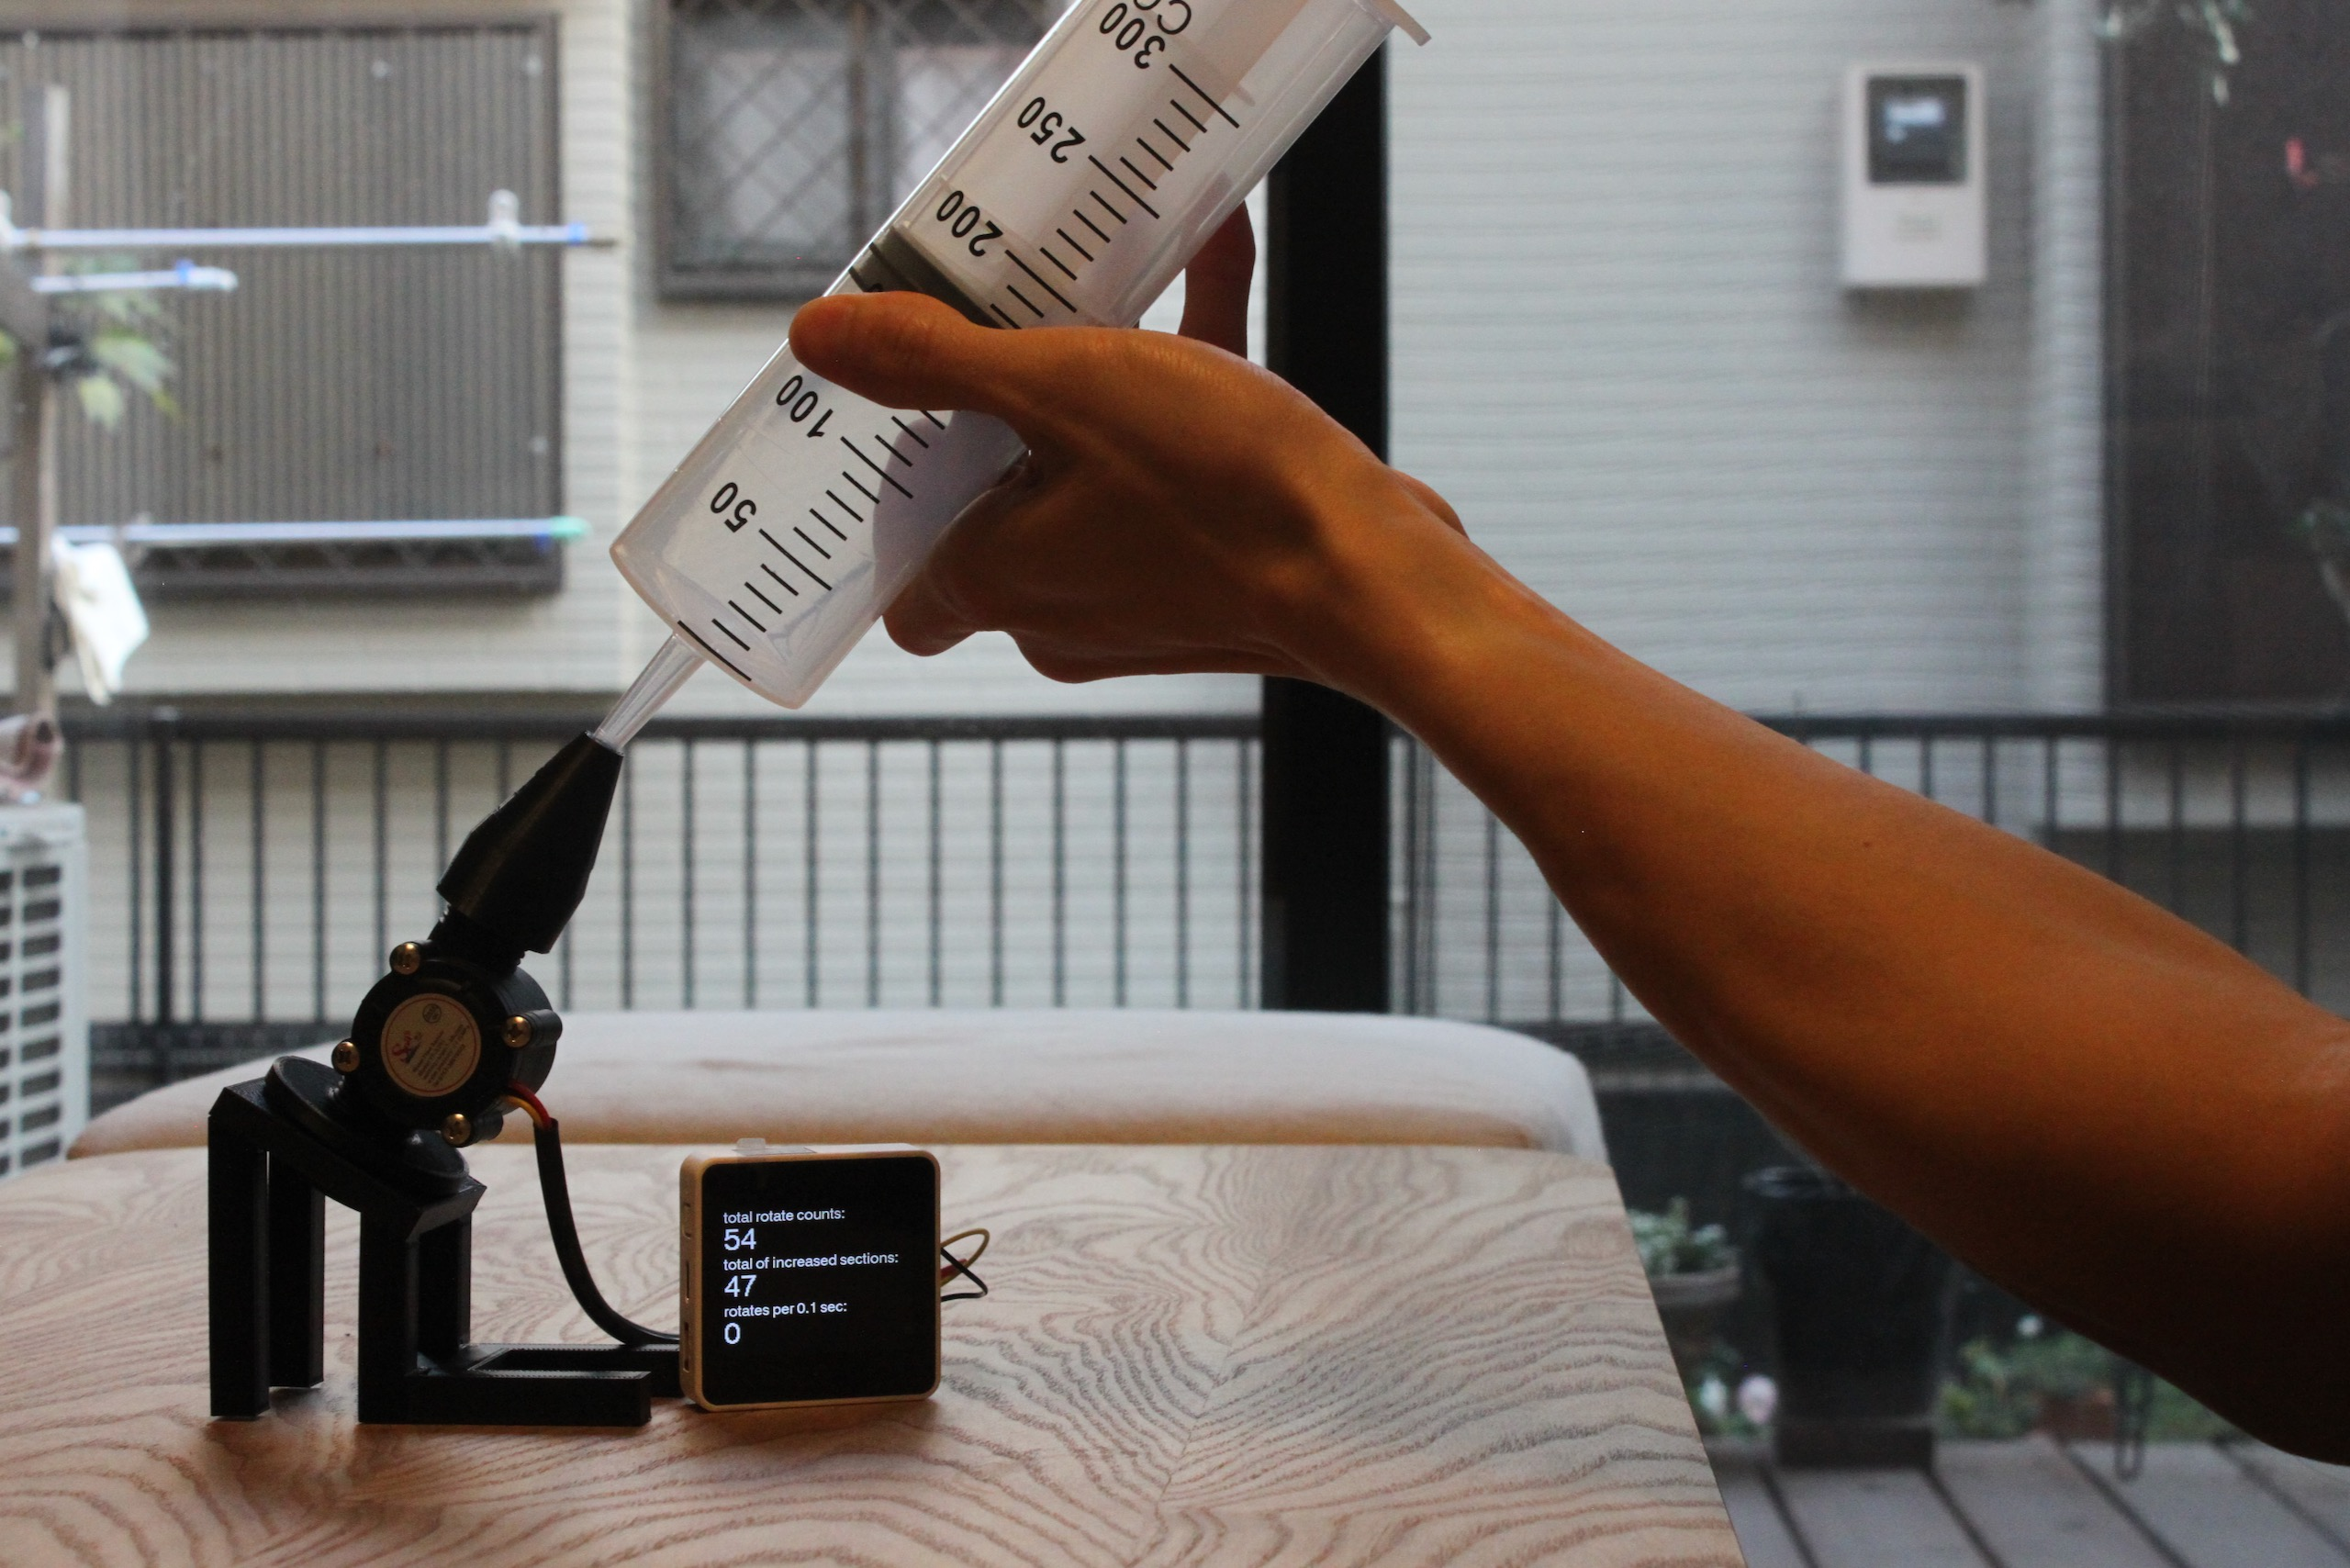
\includegraphics[width=8cm]{fig/flowsensor_calibrate}
    \caption{流量係数測定の実験}
    \label{fig:flowsensor_calibrate}
  \end{center}
\end{figure}

図\ref{fig:flowsensor_calibrate}は実験の様子である.空気の量を正確に測りとれるシリンジを水流計の入り口に接続し,一定量の空気を送り込んだ時のパルスの数を測定した.送り込む空気の量は,入手が可能であったシリンジの最大サイズから300mLとした(図\ref{fig:syringe}.シリンジのピストンを押す速さが出来る限り一定になるように注意しながら手でピストンを押した.シリンジと流量計の接続部は空気が漏れないようにするために,シリンジのノズル先端と流量計の入り口を接続する逆漏斗状のジョイント部品を3Dプリンターで製作した.ジョイント部品には,シリンジのノズルから出た高圧の空気が流量計のタービンに直撃するのを避けるため,図\ref{fig:syringe_cone}のように,ノズルから出た空気が一度中央の壁に当たって跳ね返り,周囲から水流計へと流れる形状とした.また,実際に取り付ける状態を想定して流量計の角度を60度に保つために,3Dプリンターで台座を製作した台座に置いた状態で実験を行った.

\begin{figure}[H]
  \begin{center}
    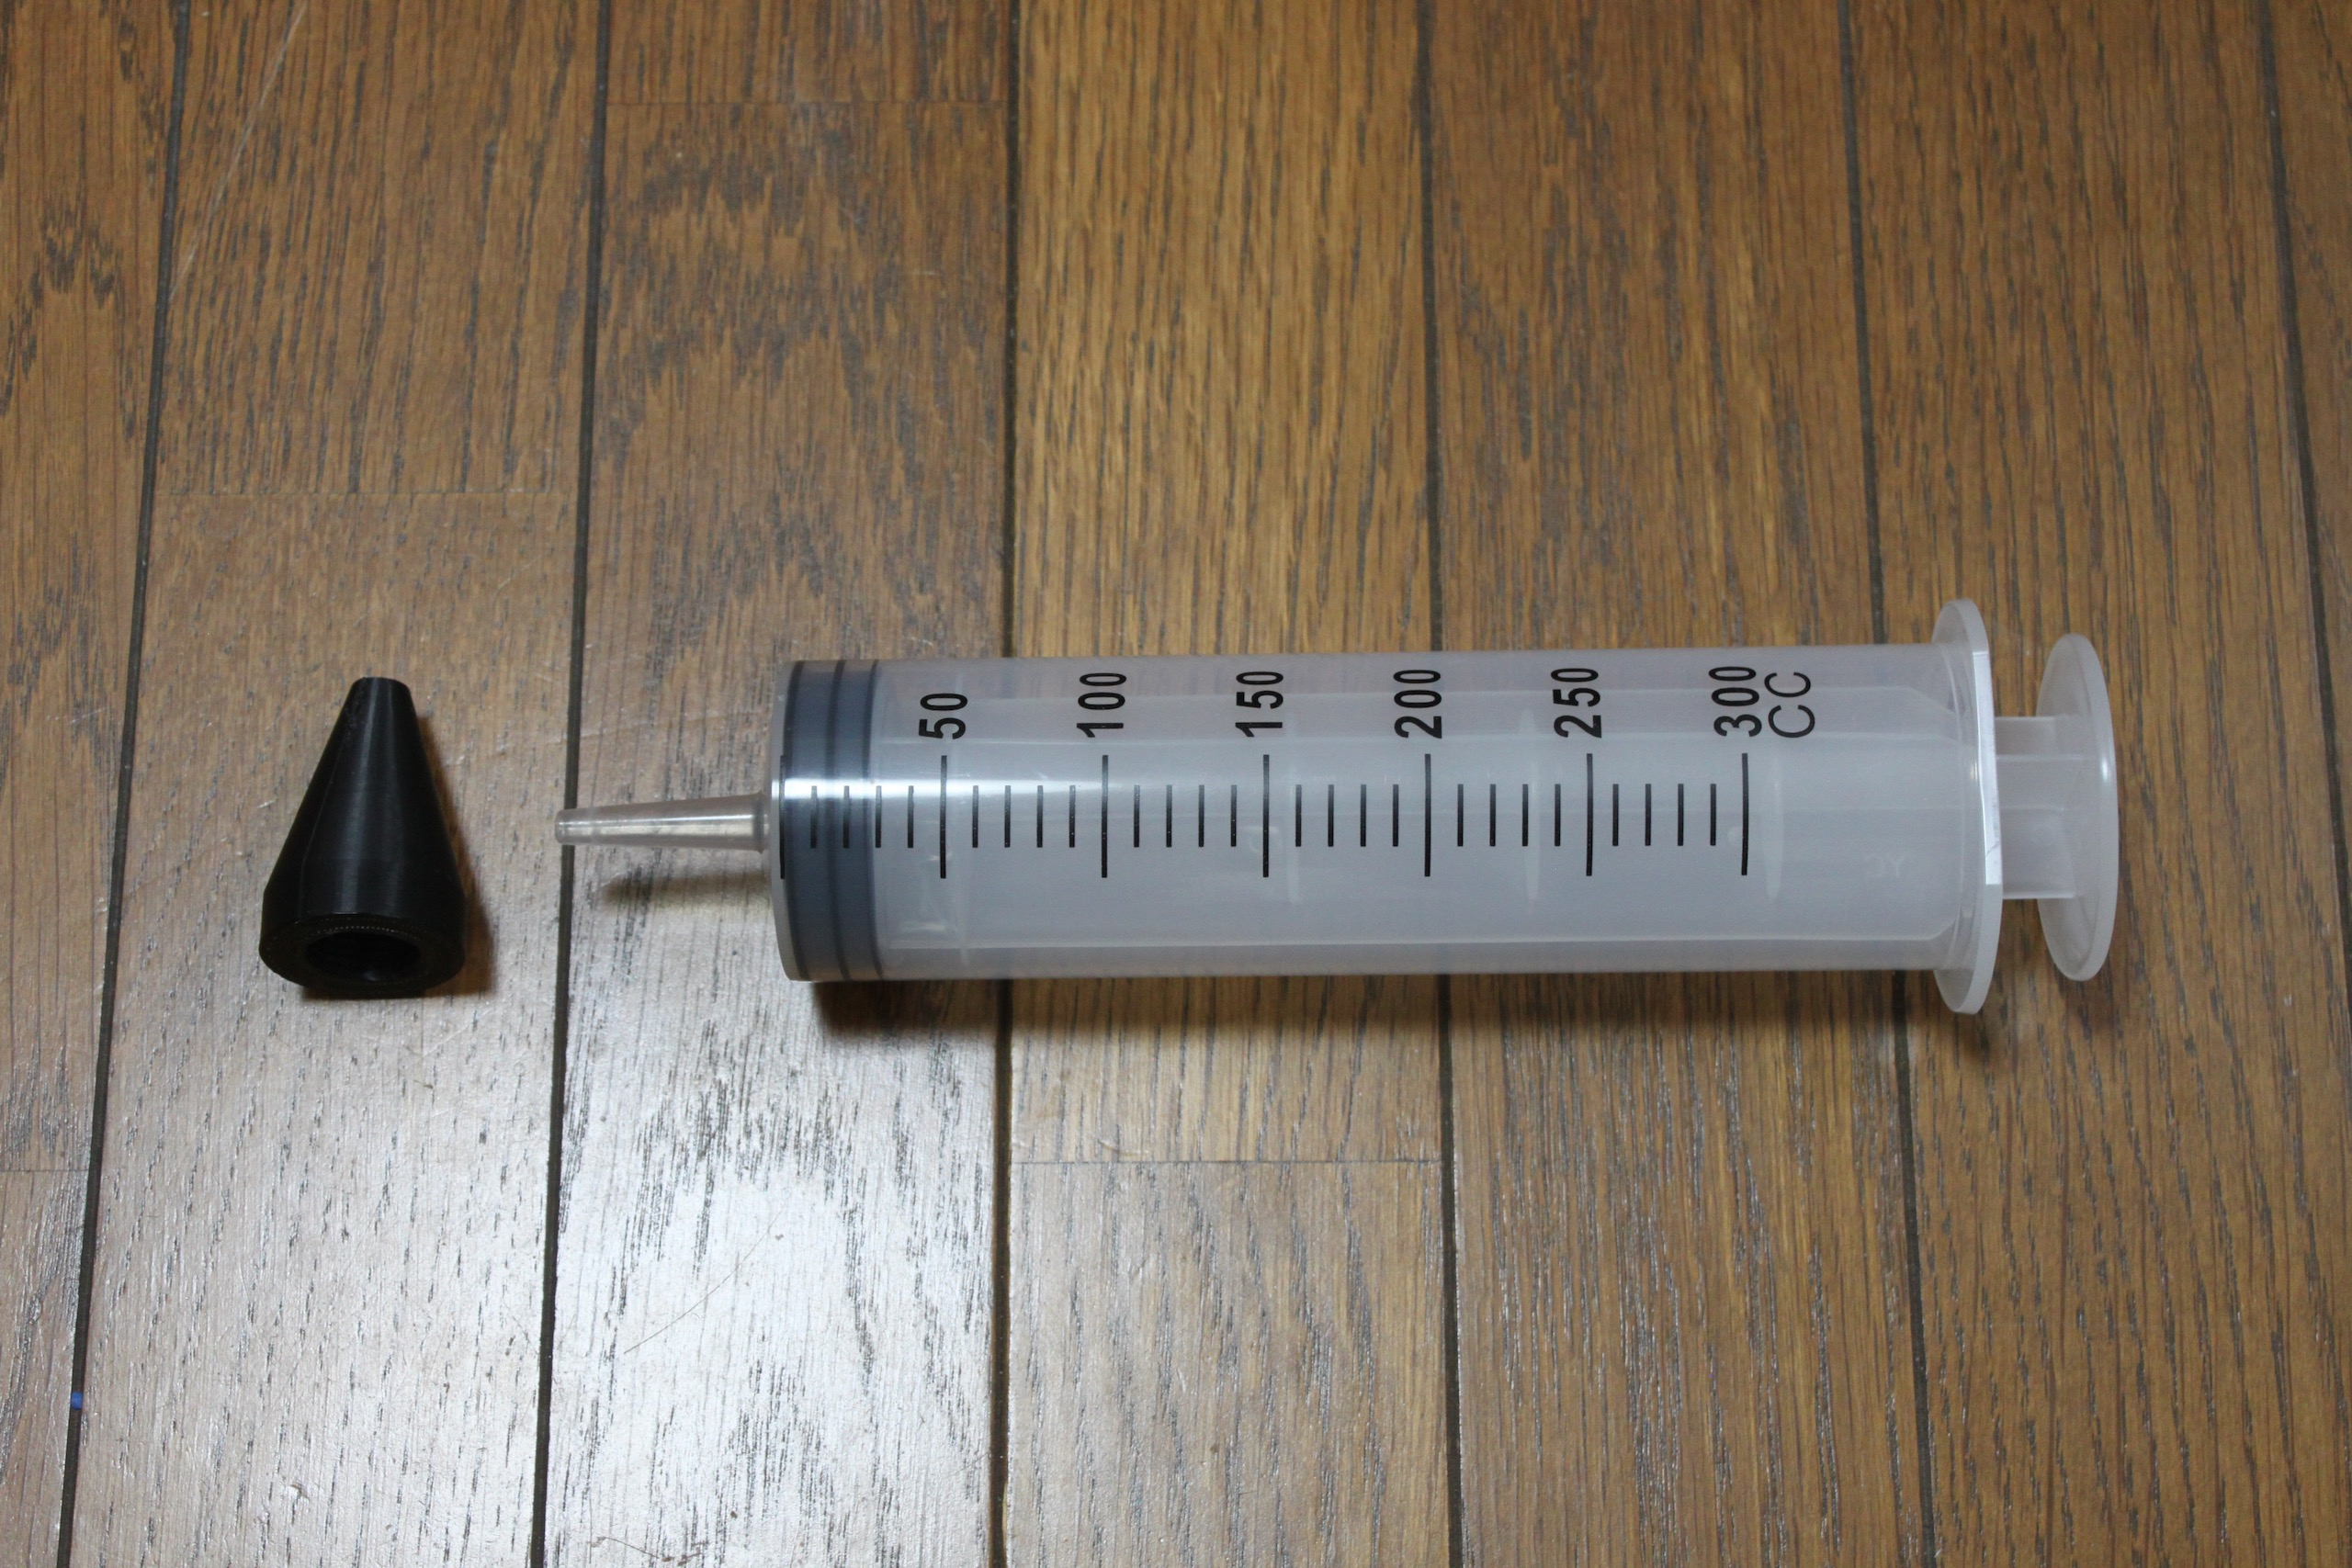
\includegraphics[width=8cm]{fig/syringe}
    \caption{接続用ジョイント部品とシリンジ}
    \label{fig:syringe}
  \end{center}
\end{figure}

\begin{figure}[H]
  \begin{center}
    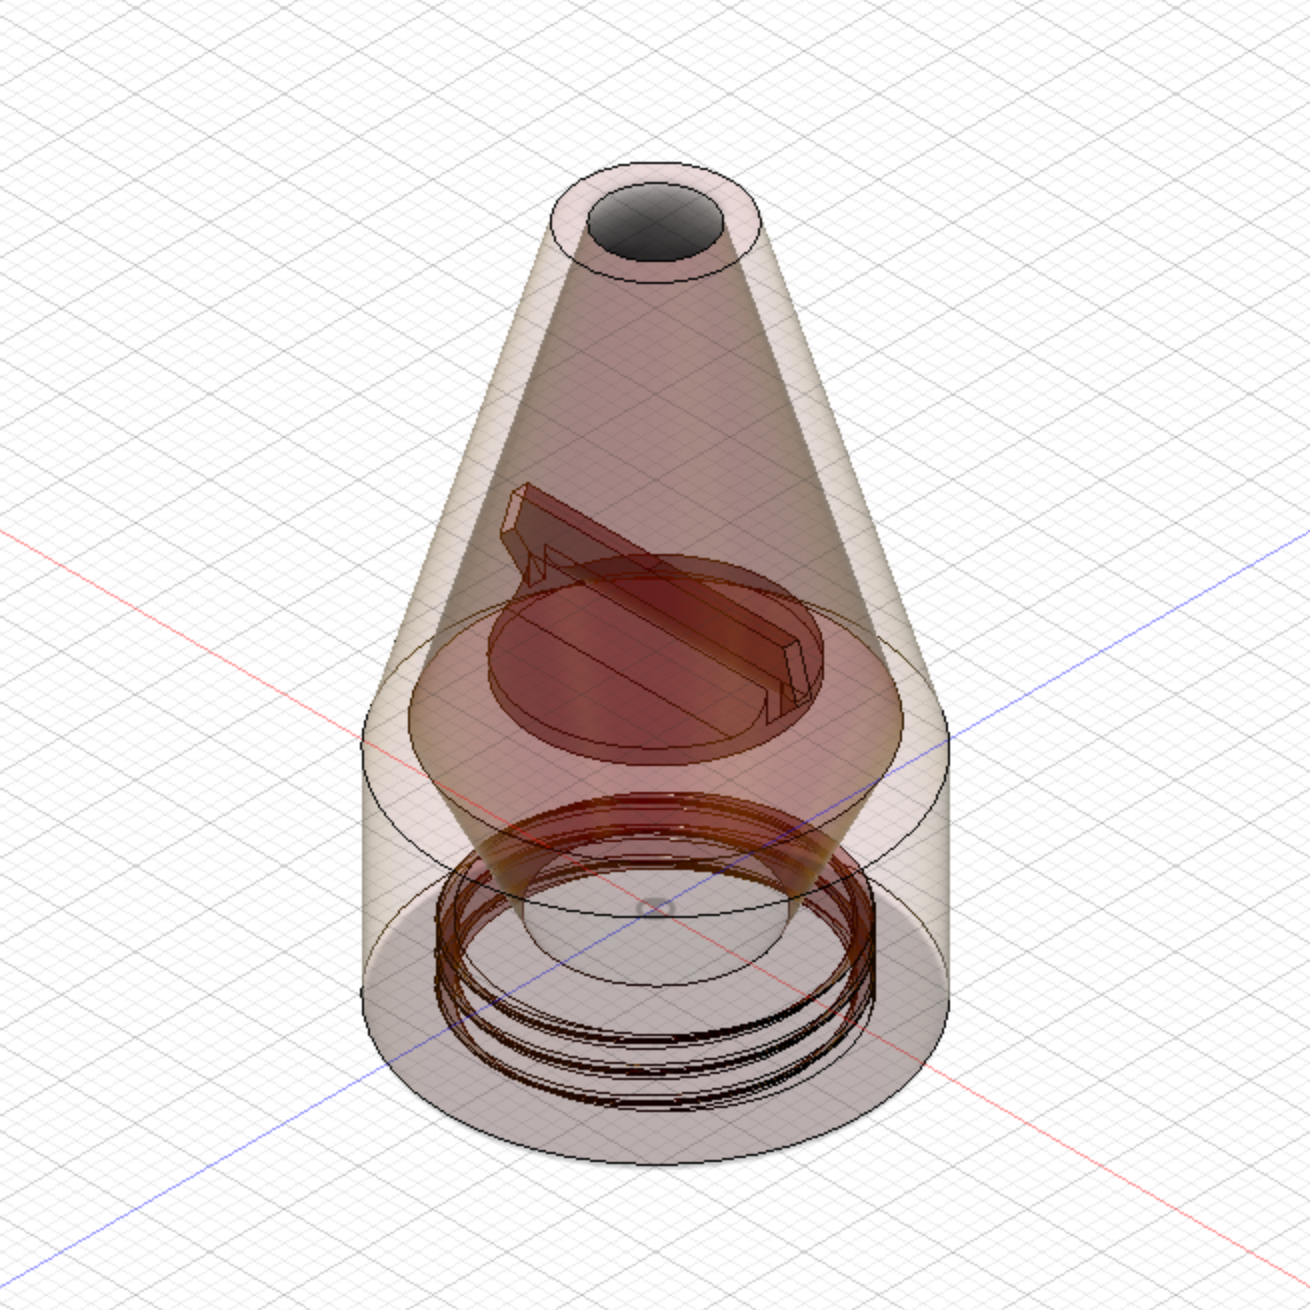
\includegraphics[width=8cm]{fig/syringe_cone}
    \caption{ジョイント部品の構造}
    \label{fig:syringe_cone}
  \end{center}
\end{figure}

今回の装置では流量計を呼気側の逆流防止弁の排気側に取り付ける.実際の呼気流量は呼気が終了し逆流防止弁が閉じた時点で0になるが,実際には流量計のタービンが空転することにより,実際には呼気が行われていない分の呼気流量を測定することとなってしまう.そこで正しく呼気流量を測定するためにはこの空転分の区間を除外する必要がある.一呼吸の内で呼気が行われ逆流防止弁が開いている間,呼気の流量は増加し続ける.このことから,流量計のタービンの時間あたりのパルス数を0.1秒ごとに算出し,これが増加から減少に転じた時間までのパルス数を係数の算出に用いた(図\ref{fig:flowsensor_increased_section}.

\begin{figure}[H]
  \begin{center}
    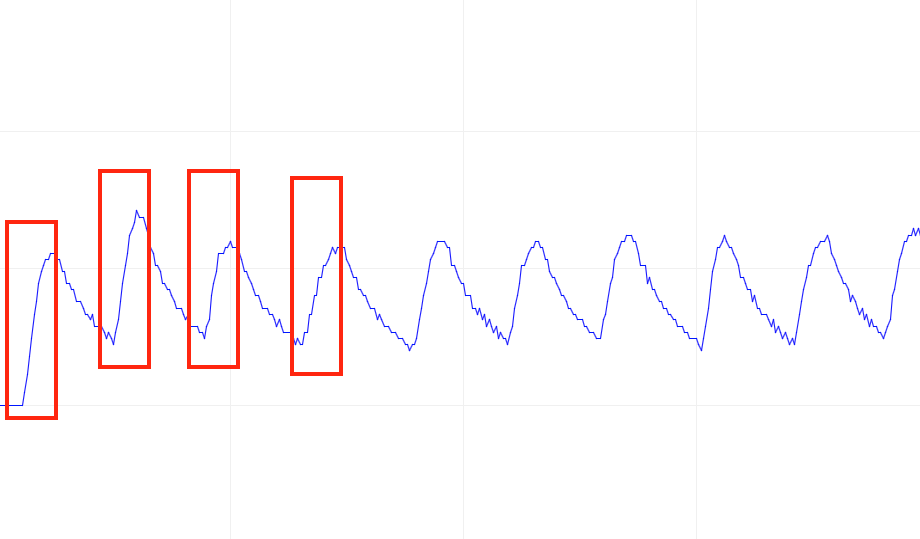
\includegraphics[width=8cm]{fig/flowsensor_increased_section}
    \caption{赤枠線で囲った部分がパルス数の増加区間}
    \label{fig:flowsensor_increased_section}
  \end{center}
\end{figure}

以上の処理を行い,空転分を除外した回転数を計測するプログラムを作成しM5Stack Core2で動作させてパルス数を測定した.上記の方法でパルス数を測定するということを200回繰り返す実験を行い

\subsubsection{信号処理}

数値計算に必要な換気量は1分値であるので,タービンの回転数の計測時間を長くすることによって誤差を減らすために1分毎に1分間の合計のタービンの回転数を係数で割った値を現在から1分前の区間の換気量としている.画面表示用の瞬間換気量は1秒毎の回転数を係数で割ったものだが,これは数値計算には用いていない.

\subsection{呼気酸素濃度の計測}

\subsubsection{空気亜鉛電池式センサー}

今回は株式会社ピーバンドットコムから発売されている「実習用酸素センサキット A-5S」(以下「A-5S」)を酸素センサーとして使用した.A-5Sは,補聴器など用に汎用的に使用される空気亜鉛電池をセンサーとして使用し,空気亜鉛電池の出力電圧から酸素濃度を測定するというセンサーで,組み立てキットとして1000円程度で購入が可能である.構造は単純であり,空気亜鉛電池に固定抵抗と可変抵抗を接続したというものである.キャリブレーションは大気中の酸素濃度20.84\%とに合わせて出力電圧が20.84mVになるように可変抵抗を調整して行う.空気亜鉛電池の電圧の低下から,長時間連続での測定は困難である.

従来,呼吸代謝測定装置の酸素センサーにはガルバニ電池式センサーが多くの場合で使われてきた.この方式は高精度であるが,酸素濃度に応じて電圧を出力することで酸素濃度を測定するためのガルバニ電池が10000円以上と高価であるため,安価に入手できる空気亜鉛電池をセンサーとして用いたA-5Sを使用した.

\subsubsection{信号処理}

A-5Sが出力する電圧は酸素濃度21\%時に21mVと非常に微弱である.この電圧を今回使用したマイコン,M5Core2(ESP32)の12bit ADコンバーター(0-3.3V, 4096段階)で測定するために,アペアンプを使用して増幅した.オペアンプには,単電源のフルスイングオペアンプNJM2732Dを用いた.非反転増幅回路を用いてA-5Sの出力電圧を101倍に増幅し,酸素濃度21\%時に2.1V程度に増幅することで測定精度を高めている.
なお,NJM2732Dは2回路入りのオペアンプであるため,接地を兼ねてもう一回路分のターミナルも結線している.現時点では呼気酸素濃度F_EO_2用の一つしか使用していないA-5Sをもう一つ追加し,吸気酸素濃度F_IO_2を計測することも可能である.

A-5Sが出力する電圧をオペアンプで増幅し,M5Stack Core2のADコンバーターで読み取ったところ,周期的にスパイク状に高い値を出力していることが確認できた.これを取り除くためにプログラム上のデジタルフィルターで信号を平滑化した.今回使用したのは移動

(回路図)

\subsection{呼気二酸化炭素の計測}

呼気二酸化炭素濃度は運動負荷によって変化し,安静時の約1\%から高強度運動時には9\%まで変化するという\cite{co2_percent}.そのため,運動中の呼吸代謝の測定にはこの範囲の二酸化炭素濃度の測定に対応する必要がある.

ところが,1万円程度以下で入手可能な市販の二酸化炭素濃度センサーは,測定範囲が0-5000ppm(0-0.5\%)のものが多い.今回は可能な限り高い運動強度での呼気二酸化炭素の濃度に対応するために,測定範囲が0-40000ppm(0-4\%)のSensirionの二酸化炭素センサーを用いたセンサーモジュールSCD30を使用した.M5Stack Core2とはI2C通信で接続を行った.表にSCD30とその仕様を示す.

SCD30はNDIR方式(非分散型赤外線吸収方式)を用いて二酸化炭素の濃度を測定する.NDIR方式は,それぞれのガスが持つ特有の吸収波長領域を利用し,特定のガスのみの濃度を測定する測定方式である.ガス濃度測定方式のうち,対象ガスに変化を及ぼすことなく濃度を測定することができるのがNDIR方式の特徴である\cite{whats_ndir}.

呼気を収集するミキシングチャンバー内は円筒形をしているため,酸素センサーA-5SとSCD30を安定して設置できるように3Dプリンターで両センサー用の台座を製作した.

%二酸化炭素濃度を測定するセンサーにはMH-Z19Bを用いた.このセンサーはNDIR方式(非分散型赤外線吸収方式)を用いて二酸化炭素の濃度を測定する.NDIR方式は,それぞれのガスが持つ特有の吸収波長領域を利用し,特定のガスのみを対象ガスに変化を及ぼすことなく濃度を測定することができるガス濃度の測定方式である\cite{whats_ndir}.MH-Z19Bは,NDIR方式の二酸化炭素濃度センサーの中でも2000-5000円程度で比較的容易に入手できるものである.

%MH-Z19Bはコマンドを送信することで二酸化炭素濃度をppm単位で容易に取得することが可能である.今回はArduino用のライブラリを用いてppm単位の二酸化炭素濃度を取得し,\%単位に変換してVCO_2の計算に使用している.

\subsection{気温・大気圧の計測}

STPD係数の算出に必要な気温・気圧は,BOSCHの温湿度・気圧センサーBME280を搭載した市販のセンサーモジュールで計測する.今回はBME280とM5Stack Core2とはI2C通信で接続を行った.BOSCH公式のほかいくつか用意されているArduino用のライブラリを用いることで,関数を用いて簡単に温度,湿度,気圧を取得することができる.今回はAdafruit製のArduinoライブラリを用いた.図および表にBME280とその仕様を示す.

センサーモジュールはM5Stack Core2が発する熱の影響を受けないように本体筐体の外側に設置した図.

\subsection{データの記録}

\subsubsection{計算用マイコン}

\subsubsection{プログラム}

\expandafter\ifx\csname ifdraft\endcsname\relax
  \end{document}
\fi
